% ============================================================
% HSBI Beamer — ISLP Lecture Series — IMPROVED EDITION
% Chapter 0: Precourse Refresher (prerequisites from undergraduate study)
% ============================================================
\documentclass[aspectratio=169,11pt]{beamer}
\usepackage[utf8]{inputenc}\usepackage[T1]{fontenc}\usepackage[english]{babel}
\usepackage{graphicx}\usepackage{booktabs}\usepackage{amsmath,amssymb,amsfonts}
\usepackage{mathtools}\usepackage{hyperref}\usepackage{xcolor}
\usepackage{verbatim}\usepackage{alltt}
\usepackage{tikz}\usetikzlibrary{calc,arrows.meta,positioning,shapes}
\usepackage{tcolorbox}\tcbuselibrary{skins}
\usepackage{textcomp}\providecommand{\euro}{\texteuro}

\usetheme{Madrid}\usecolortheme{default}
\setbeamertemplate{navigation symbols}{}
\setbeamertemplate{footline}[frame number]
\setbeamertemplate{blocks}[rounded][shadow=false]
\setbeamertemplate{headline}{%
  \leavevmode\hbox{%
    \begin{beamercolorbox}[wd=\paperwidth,ht=2.2ex,dp=0.9ex]{section in head/foot}%
      {\fontsize{4.6}{5.2}\selectfont%
       \insertsectionnavigationhorizontal{\paperwidth}{}{\hskip0pt plus1filll}}%
    \end{beamercolorbox}}%
}
\setbeamerfont{section in head/foot}{size=\tiny}
\setbeamerfont{palette primary}{size=\tiny}
\setbeamerfont{palette tertiary}{size=\tiny}
\setbeamerfont{section in toc}{size=\footnotesize}

\usepackage{listings}
\definecolor{pyKw}{RGB}{0,0,180}\definecolor{pyStr}{RGB}{20,120,40}
\definecolor{pyCom}{RGB}{120,120,120}\definecolor{accent}{RGB}{38,70,140}
\lstdefinestyle{Pystyle}{language=Python,basicstyle=\ttfamily\footnotesize,
  keywordstyle=\color{pyKw}\bfseries,commentstyle=\color{pyCom}\itshape,
  stringstyle=\color{pyStr},showstringspaces=false,upquote=true,
  columns=fullflexible,breaklines=true,literate={~}{{$\sim$}}1}
\lstset{style=Pystyle}

\AtBeginSection[]{\begin{frame}{Outline}\scriptsize
  \begin{columns}[t]
    \begin{column}{0.5\textwidth}
      \tableofcontents[currentsection,sectionstyle=show/shaded,
                       subsectionstyle=show/show/hide,sections={1-6}]
    \end{column}
    \begin{column}{0.5\textwidth}
      \tableofcontents[currentsection,sectionstyle=show/shaded,
                       subsectionstyle=show/show/hide,sections={7-12}]
    \end{column}
  \end{columns}
\end{frame}}

\newcommand{\islpsource}[1]{%
  \vfill\hfill{\tiny\itshape\color{gray}Source: #1 \textemdash{} ISLP, James et al.\ (2023).}\par
}

\newtcolorbox{takeaway}[1][Takeaway]{enhanced,colback=green!4,colframe=green!50!black,
  boxrule=0pt,leftrule=2.5pt,arc=2pt,fonttitle=\bfseries,title=#1,
  left=2mm,right=2mm,top=1mm,bottom=1mm}
\newtcolorbox{numexample}[1][Worked example]{enhanced,colback=orange!4,colframe=orange!70!black,
  boxrule=0pt,leftrule=2.5pt,arc=2pt,fonttitle=\bfseries,title=#1,
  left=2mm,right=2mm,top=1mm,bottom=1mm}
\newtcolorbox{readme}[1][How to read this]{enhanced,colback=blue!4,colframe=accent,
  boxrule=0pt,leftrule=2.5pt,arc=2pt,fonttitle=\bfseries,title=#1,
  left=2mm,right=2mm,top=1mm,bottom=1mm}

\title{Quantitative Research Methods}
\subtitle{Chapter 0: Precourse Refresher}
\author{Prof.\ Dr.\ Christoph Weisser}\institute{HSBI}
\date{Summer Semester 2026}\graphicspath{{images/}}

\newtcolorbox{exercise}[1][Exercise]{enhanced, fontupper=\footnotesize, colback=purple!4, colframe=purple!55!black, boxrule=0pt, leftrule=2.5pt, arc=2pt, fonttitle=\bfseries, title=#1, left=2mm, right=2mm, top=1mm, bottom=1mm}
\newtcolorbox{solutionbox}[1][Solution]{enhanced, fontupper=\footnotesize, colback=teal!5, colframe=teal!55!black, boxrule=0pt, leftrule=2.5pt, arc=2pt, fonttitle=\bfseries, title=#1, left=2mm, right=2mm, top=1mm, bottom=1mm}

% Reclaim ~2pt of body height (custom nav headline makes full slides tip over by ~1.83pt)
\addtobeamertemplate{frametitle}{}{\vspace{-2pt}}

\newtcolorbox{longexercise}[1][Extended exercise (15 min)]{enhanced, fontupper=\footnotesize, colback=violet!6, colframe=violet!55!black, boxrule=0pt, leftrule=3pt, arc=2pt, fonttitle=\bfseries, title=#1, left=2mm, right=2mm, top=1mm, bottom=1mm}

\newtcolorbox{labnote}[1][Run this live in the lab notebook]{enhanced, fontupper=\footnotesize, colback=cyan!7, colframe=cyan!45!black, boxrule=0pt, leftrule=3pt, arc=2pt, fonttitle=\bfseries, title=#1, left=2mm, right=2mm, top=1mm, bottom=1mm}

\begin{document}
\begin{frame}[plain]\titlepage\end{frame}

\begin{frame}{The course at a glance}
  \footnotesize
  \begin{center}
  \begin{tabular}{@{}c r l@{}}
    & \textbf{Lecture} & \textbf{Topic}\\
    \midrule
    $\blacktriangleright$ & \textbf{0} & \textbf{Precourse --- refresher of undergraduate statistics, algebra, Python} \\
     & 1 & Ch.\ 1 + 2 --- Introduction; what is statistical learning \\
     & 2 & Ch.\ 2 --- Accuracy, bias--variance, Bayes classifier, KNN \\
     & 3--4 & Ch.\ 3 --- Linear regression (estimation, inference, diagnostics) \\
     & 5--6 & Ch.\ 4 --- Classification (logistic, LDA/QDA, naive Bayes, ROC) \\
     & 7 & Ch.\ 5 --- Resampling (validation, CV, bootstrap) \\
     & 8 & Ch.\ 6 --- Model selection and regularisation (ridge, lasso) \\
     & 9 & Ch.\ 7 --- Moving beyond linearity (splines, GAMs) \\
     & 10 & Ch.\ 8 --- Tree-based methods (trees, forests, boosting) \\
     & 11 & Ch.\ 10 --- Deep learning (MLPs, CNNs, training) \\
     & 12 & Ch.\ 13 --- Multiple testing (FWER, FDR) \\
  \end{tabular}
  \end{center}
  \vspace{2pt}
  {\scriptsize This refresher is \emph{optional} and sits before Lecture 1. It assumes nothing
  beyond an introductory undergraduate course, and it only covers material the
  twelve lectures actually rely on. $\blacktriangleright$ marks today's session.}
\end{frame}

\begin{frame}{Contents}
  \begin{columns}[t]
    \begin{column}{0.5\textwidth}
      \tableofcontents[hideallsubsections,sections={1-6}]
    \end{column}
    \begin{column}{0.5\textwidth}
      \tableofcontents[hideallsubsections,sections={7-12}]
    \end{column}
  \end{columns}
\end{frame}

\begin{frame}{Notation in this refresher}
  \footnotesize
  \begin{center}
  \begin{tabular}{@{}ll@{}}
    \toprule
    \textbf{Symbol} & \textbf{Meaning} \\
    \midrule
    $n$, $p$ & number of observations; number of variables \\
    $x_i$, $y_i$ & predictor and response value of observation $i$ \\
    $\bar x$, $s$, $s^2$ & sample mean, sample standard deviation, sample variance \\
    $\mu$, $\sigma$, $\sigma^2$ & population mean, standard deviation, variance \\
    $Q_1, Q_3$, IQR & lower/upper quartile; interquartile range $Q_3-Q_1$ \\
    $r$ & sample correlation coefficient \\
    $\mathrm{Cov}(X,Y)$ & covariance of two random variables \\
    $\mathrm{E}[X]$, $\mathrm{Var}(X)$ & expected value and variance of $X$ \\
    $\hat\theta$ & an estimate of the unknown quantity $\theta$ (``hat'' = estimated) \\
    $\mathrm{SE}(\hat\theta)$ & standard error: the SD of $\hat\theta$ across repeated samples \\
    $H_0$, $H_1$ & null and alternative hypothesis \\
    $\alpha$ & significance level (tolerated false-positive rate) \\
    $\mathbf{X}$, $\mathbf{y}$ & $n\times p$ data matrix; $n$-vector of responses \\
    $\boldsymbol\beta$, $\hat{\boldsymbol\beta}$ & vector of true / estimated regression coefficients \\
    $\nabla f$ & gradient: the vector of partial derivatives of $f$ \\
    \bottomrule
  \end{tabular}
  \end{center}
\end{frame}

\begin{frame}{Why a refresher, and how to use it}
  \begin{takeaway}[The purpose]
    This course does not teach statistics from scratch --- it teaches
    \emph{statistical learning}. Everything here is assumed known from
    Lecture 1 onwards. One session, so that nobody is stuck on notation
    while we discuss the ideas that matter.
  \end{takeaway}
  \begin{readme}[How to use it]
    \begin{itemize}
      \item If a slide is obvious to you, that topic is fine --- move on.
      \item If a slide is new, work its exercise before Lecture 1.
      \item Each section ends with \emph{where this reappears in the course},
            so you can see why it is worth the effort.
    \end{itemize}
  \end{readme}
\end{frame}

\begin{frame}{Learning objectives for this refresher}
  By the end of this session you will be able to:
  \begin{itemize}
    \item \textbf{Classify} variables by type and choose an appropriate summary
          and plot for each.
    \item \textbf{Compute and interpret} mean, median, variance, SD, quartiles,
          IQR, covariance and correlation.
    \item \textbf{Apply} the rules of probability, conditional probability and
          Bayes' theorem, and use expectation and variance rules.
    \item \textbf{Recognise} the normal, $t$, $\chi^2$, $F$, Bernoulli, binomial
          and Poisson distributions and say where each is used.
    \item \textbf{Explain} sampling variability, standard errors, confidence
          intervals and $p$-values --- and their standard misreadings.
    \item \textbf{Fit and interpret} a simple linear regression by hand.
    \item \textbf{Manipulate} vectors and matrices, and read the matrix form of
          the regression estimator.
    \item \textbf{Differentiate} a loss function and take a gradient-descent step.
    \item \textbf{Use} \texttt{numpy}, \texttt{pandas} and \texttt{matplotlib} for
          the basic tasks of the labs.
  \end{itemize}
\end{frame}

\begin{frame}{Do you actually need this session? A 10-question self-check}
  \footnotesize
  Answer honestly. Each question maps to one section of this deck.
  \begin{enumerate}
    \item Why is the median often reported for income, but the mean for test scores?
    \item What does it mean that a variable has SD $=0$?
    \item Two variables have $r = 0$. Can they still be strongly related?
    \item A test is 99\% accurate and you test positive. Is there a 99\% chance
          you are ill?
    \item What is the difference between a standard deviation and a standard error?
    \item What exactly is ``95\%'' about a 95\% confidence interval?
    \item A $p$-value of $0.03$: what is the probability that $H_0$ is true?
    \item In $\hat y = 2 + 3x$, what does the $3$ mean --- in words, with units?
    \item What are the dimensions of $\mathbf{X}^\top\mathbf{X}$ if $\mathbf{X}$
          is $n \times p$?
    \item What does the derivative of a loss function tell an optimisation
          algorithm to do?
  \end{enumerate}
  \begin{takeaway}[Scoring]
    Comfortable with 8+? Skim this deck. Fewer than 5? Work through it with the
    exercises --- it will pay for itself by Lecture 3.
  \end{takeaway}
\end{frame}

\begin{frame}{Sources and references}
  \begin{block}{Primary textbook (from Lecture 1 onwards)}
    James, G., Witten, D., Hastie, T., Tibshirani, R., \& Taylor, J.\ (2023).
    \emph{An Introduction to Statistical Learning, with Applications in
    Python.} Springer. Chapter 2 and the Chapter 3 appendix cover much of
    this refresher in condensed form.
  \end{block}
  \begin{block}{If you want a fuller undergraduate treatment}
    Any introductory statistics text will do; the topics to look up are listed
    on the final ``where to read more'' slide. All figures in this deck were
    computed from the course data sets.
  \end{block}
\end{frame}


% ============================================================
\section{Data, variables and notation}
% ============================================================

\begin{frame}{Roadmap of this refresher}
  \begin{takeaway}[How this session is organised]
    \begin{enumerate}
      \item Data, variables and notation --- the language.
      \item Describing one variable, then two.
      \item Probability, random variables and the standard distributions.
      \item Sampling, estimation, confidence intervals, hypothesis tests.
      \item Simple linear regression --- the bridge into Chapter 3.
      \item The linear algebra and calculus the later chapters use.
      \item The Python toolkit of the labs.
    \end{enumerate}
  \end{takeaway}
  Roughly one exercise every 20 minutes; solutions follow immediately.
\end{frame}

\begin{frame}{The shape of a data set: $n$ observations, $p$ variables}
  \begin{center}
    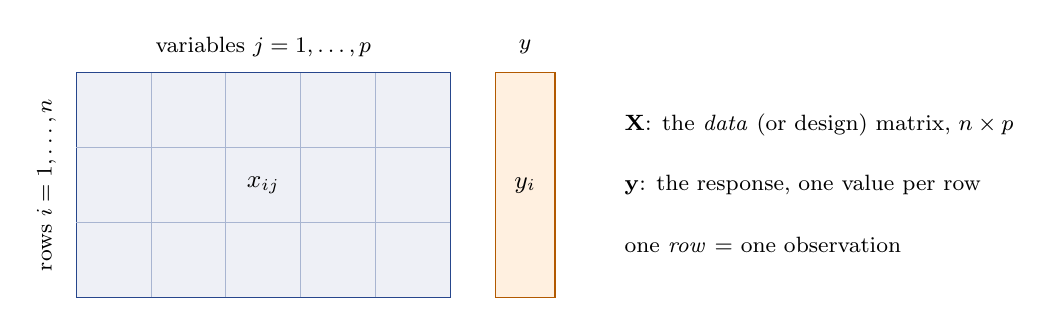
\begin{tikzpicture}[scale=0.95]
      \draw[fill=accent!8,draw=accent] (0,0) rectangle (5,3);
      \foreach \i in {1,...,4} \draw[accent!40] (\i,0) -- (\i,3);
      \foreach \j in {1,...,2} \draw[accent!40] (0,\j) -- (5,\j);
      \node at (2.5,3.35) {\footnotesize variables $j = 1,\dots,p$};
      \node[rotate=90] at (-0.4,1.5) {\footnotesize rows $i = 1,\dots,n$};
      \node at (2.5,1.5) {\small $x_{ij}$};
      \draw[fill=orange!12,draw=orange!70!black] (5.6,0) rectangle (6.4,3);
      \node at (6.0,3.35) {\footnotesize $y$};
      \node at (6.0,1.5) {\small $y_i$};
      \node[align=left,anchor=west] at (7.2,2.3)
        {\footnotesize $\mathbf{X}$: the \emph{data} (or design) matrix, $n\times p$};
      \node[align=left,anchor=west] at (7.2,1.5)
        {\footnotesize $\mathbf{y}$: the response, one value per row};
      \node[align=left,anchor=west] at (7.2,0.7)
        {\footnotesize one \emph{row} $=$ one observation};
    \end{tikzpicture}
  \end{center}
  \begin{takeaway}[Tidy data]
    One row per observational unit, one column per variable, one value per
    cell. Every method in this course expects data in this shape.
  \end{takeaway}
\end{frame}

\begin{frame}{Variable types decide everything that follows}
  \begin{center}
    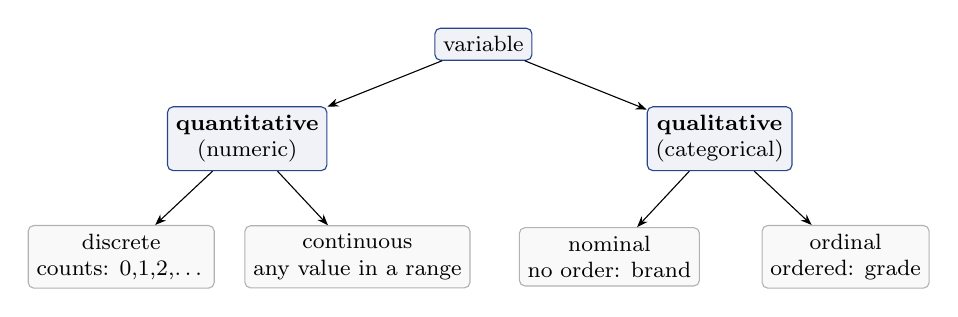
\begin{tikzpicture}[
      every node/.style={font=\footnotesize},
      box/.style={draw=accent,fill=accent!7,rounded corners=2pt,inner sep=3pt,align=center},
      lvl/.style={draw=gray!60,fill=gray!5,rounded corners=2pt,inner sep=3pt,align=center},
      ->,>={Stealth[length=4pt]}]
      \node[box] (v) at (0,2.6) {variable};
      \node[box] (q) at (-3,1.4) {\textbf{quantitative}\\(numeric)};
      \node[box] (c) at (3,1.4) {\textbf{qualitative}\\(categorical)};
      \node[lvl] (disc) at (-4.6,-0.1) {discrete\\counts: 0,1,2,\dots};
      \node[lvl] (cont) at (-1.6,-0.1) {continuous\\any value in a range};
      \node[lvl] (nom) at (1.6,-0.1) {nominal\\no order: brand};
      \node[lvl] (ord) at (4.6,-0.1) {ordinal\\ordered: grade};
      \draw (v) -- (q); \draw (v) -- (c);
      \draw (q) -- (disc); \draw (q) -- (cont);
      \draw (c) -- (nom); \draw (c) -- (ord);
    \end{tikzpicture}
  \end{center}
  \footnotesize
  \begin{tabular}{@{}lll@{}}
    \toprule
    \textbf{Type} & \textbf{Summarise with} & \textbf{Plot with} \\
    \midrule
    Quantitative & mean, SD, median, quartiles & histogram, boxplot, scatter \\
    Qualitative & counts, proportions & bar chart, contingency table \\
    \bottomrule
  \end{tabular}
\end{frame}

\begin{frame}{Why the type matters in this course}
  \begin{takeaway}[The single most consequential distinction]
    The \emph{response} type names the problem:
    \begin{itemize}
      \item quantitative $y$ $\Rightarrow$ \textbf{regression} (Ch.\ 3, 6, 7),
      \item qualitative $y$ $\Rightarrow$ \textbf{classification} (Ch.\ 4, 8, 10).
    \end{itemize}
  \end{takeaway}
  \begin{readme}[Qualitative \emph{predictors} are not a problem]
    A categorical predictor enters as \emph{dummy} (0/1) variables --- one
    fewer than the number of categories, so ``brand'' with 3 levels costs 2
    columns of $\mathbf{X}$, not 1 (Chapter 3).
  \end{readme}
  \begin{numexample}[From the course data]
    \texttt{Wage}: \texttt{wage} is quantitative (regression, Ch.\ 7).
    \texttt{Default}: \texttt{default} is Yes/No (classification, Ch.\ 4).
    \texttt{Smarket}: \texttt{Direction} is Up/Down (classification, Ch.\ 4).
  \end{numexample}
\end{frame}

\begin{frame}{Population and sample: the loop this whole course lives in}
  \begin{center}
    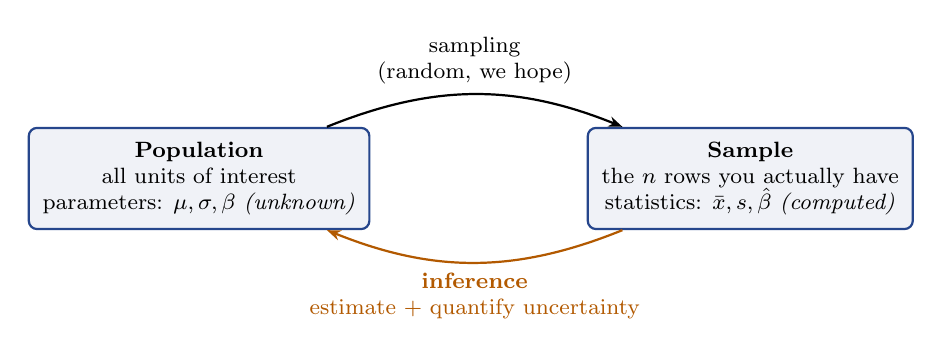
\begin{tikzpicture}[every node/.style={font=\footnotesize},
      b/.style={draw=accent,fill=accent!7,rounded corners=3pt,inner sep=5pt,align=center},
      ->,>={Stealth[length=5pt]},thick]
      \node[b] (pop) at (0,0) {\textbf{Population}\\all units of interest\\parameters: $\mu,\sigma,\beta$ \emph{(unknown)}};
      \node[b] (sam) at (7,0) {\textbf{Sample}\\the $n$ rows you actually have\\statistics: $\bar x, s, \hat\beta$ \emph{(computed)}};
      \draw[->] (pop) to[bend left=22] node[above,align=center]{sampling\\(random, we hope)} (sam);
      \draw[->,orange!70!black] (sam) to[bend left=22] node[below,align=center]{\textbf{inference}\\estimate + quantify uncertainty} (pop);
    \end{tikzpicture}
  \end{center}
  \begin{takeaway}[Greek vs.\ Latin --- and hats]
    Greek letters ($\mu$, $\sigma$, $\beta$) denote unknown \emph{population}
    quantities; Latin letters and hats ($\bar x$, $s$, $\hat\beta$) denote
    things \emph{computed from data}. A hat always means ``estimated''.
  \end{takeaway}
\end{frame}

\begin{frame}{Exercise 0.1 --- Variable types and summaries [Concept]}
  \begin{exercise}
    A university records, for each of $n$ students: degree programme
    (Business, Engineering, Law); age in years; number of exam attempts;
    satisfaction on a 1--5 scale (1 = very poor, \dots, 5 = very good);
    and starting salary in euros.
    \begin{enumerate}
      \item Classify each of the five variables as quantitative (discrete /
            continuous) or qualitative (nominal / ordinal).
      \item For each, name one appropriate numerical summary and one plot.
      \item The university wants to predict starting salary. Is this a
            regression or a classification problem? What if it instead wants
            to predict whether a student graduates on time?
      \item Someone computes the mean of ``degree programme'' by coding
            Business $=1$, Engineering $=2$, Law $=3$, and reports $1.8$.
            What is wrong with this?
    \end{enumerate}
  \end{exercise}
\end{frame}

\begin{frame}{Solution --- Exercise 0.1}
  \begin{solutionbox}
    \textbf{(1) and (2).}
    \begin{center}\scriptsize
    \begin{tabular}{@{}llll@{}}
      \toprule
      \textbf{Variable} & \textbf{Type} & \textbf{Summary} & \textbf{Plot} \\
      \midrule
      Degree programme & qualitative, nominal & counts / proportions & bar chart \\
      Age & quantitative, continuous & mean and SD (or median, IQR) & histogram, boxplot \\
      Exam attempts & quantitative, discrete & mean, or median (skewed) & bar chart of counts \\
      Satisfaction & qualitative, ordinal & median, quartiles & bar chart \\
      Starting salary & quantitative, continuous & \emph{median} (right-skewed) & histogram, boxplot \\
      \bottomrule
    \end{tabular}
    \end{center}
    \textbf{(3).} Salary is quantitative $\Rightarrow$ \textbf{regression}.
    ``Graduates on time'' is Yes/No $\Rightarrow$ \textbf{classification}.
    The data are the same; the \emph{response type} names the problem.

    \textbf{(4).} The codes 1, 2, 3 are arbitrary labels, not quantities:
    Law is not ``three times'' Business, and the gaps are not equal or even
    meaningful. The mean $1.8$ therefore has no interpretation --- it would
    change if the categories were relabelled. Summarise nominal variables by
    counts and proportions. (In a model, such a variable becomes dummy
    variables, not a single numeric column.)
  \end{solutionbox}
\end{frame}


% ============================================================
\section{Describing one variable}
% ============================================================

\begin{frame}{Three questions to ask of any single variable}
  \begin{takeaway}[Centre --- spread --- shape]
    \begin{enumerate}
      \item \textbf{Centre}: where do typical values sit? (mean, median, mode)
      \item \textbf{Spread}: how much do values differ? (SD, variance, range, IQR)
      \item \textbf{Shape}: symmetric or skewed, one peak or several, outliers?
    \end{enumerate}
    Never report a centre without a spread. ``Average salary $=\,$\euro 52{,}000''
    means something quite different with SD \euro 3{,}000 than with SD \euro 40{,}000.
  \end{takeaway}
  \begin{readme}[Why the shape decides the summary]
    For symmetric data, mean and SD say it all. For skewed data (income,
    house prices, waiting times) the mean is dragged by the tail --- report
    the median and IQR as well.
  \end{readme}
\end{frame}

\begin{frame}{Measures of centre}
  \begin{block}{Definitions}
    \[
      \bar x = \frac{1}{n}\sum_{i=1}^{n} x_i,
      \qquad
      \text{median} = \text{the middle value of the sorted data},
      \qquad
      \text{mode} = \text{the most frequent value.}
    \]
  \end{block}
  \footnotesize
  \begin{tabular}{@{}lll@{}}
    \toprule
    \textbf{Measure} & \textbf{Use when} & \textbf{Weakness} \\
    \midrule
    Mean $\bar x$ & data roughly symmetric; algebra needed & pulled by outliers \\
    Median & data skewed or outlier-prone & ignores magnitudes; harder algebra \\
    Mode & categorical data; finding peaks & may not be unique or exist \\
    \bottomrule
  \end{tabular}
  \begin{takeaway}[The mean is the balance point]
    $\sum_i (x_i - \bar x) = 0$ always: deviations above and below the mean
    cancel exactly. This identity is why squared deviations, not raw ones,
    are used to measure spread --- and it reappears as the ``residuals sum to
    zero'' property in Chapter 3.
  \end{takeaway}
\end{frame}

\begin{frame}{Measures of spread}
  \footnotesize
  \begin{block}{Sample variance and standard deviation}
    \[
      s^2 = \frac{1}{n-1}\sum_{i=1}^{n}(x_i - \bar x)^2,
      \qquad
      s = \sqrt{s^2}.
    \]
  \end{block}
  \begin{readme}[Reading it symbol by symbol]
    $(x_i - \bar x)$ is how far observation $i$ sits from the centre; squaring
    removes the sign and penalises large deviations; summing aggregates;
    dividing averages. The square root returns to the original units --- which
    is why $s$, not $s^2$, is the number you report.
  \end{readme}
  \begin{takeaway}[Why $n-1$ and not $n$?]
    One degree of freedom was spent estimating $\bar x$ from the same data;
    dividing by $n-1$ makes $s^2$ unbiased for $\sigma^2$. The same
    bookkeeping returns in the $t$- and $F$-tests and in the
    effective-degrees-of-freedom arguments of Chapters 5--7.
  \end{takeaway}
\end{frame}

\begin{frame}{Quantiles, the five-number summary, and the boxplot}
  \begin{center}
    
\includegraphics[width=0.86\textwidth,height=0.56\textheight,keepaspectratio]{ch00_boxplot_anatomy.png}
  \end{center}
  \footnotesize
  The $q$-quantile is the value below which a fraction $q$ of the data lies.
  $Q_1 = 25\%$, median $=50\%$, $Q_3 = 75\%$; $\mathrm{IQR} = Q_3 - Q_1$ holds
  the middle half. The usual outlier rule flags points outside
  $[\,Q_1 - 1.5\,\mathrm{IQR},\ Q_3 + 1.5\,\mathrm{IQR}\,]$ --- a convention,
  not a law, and never a licence to delete data.
\end{frame}

\begin{frame}{Shape: skewness read off a picture}
  \begin{center}
    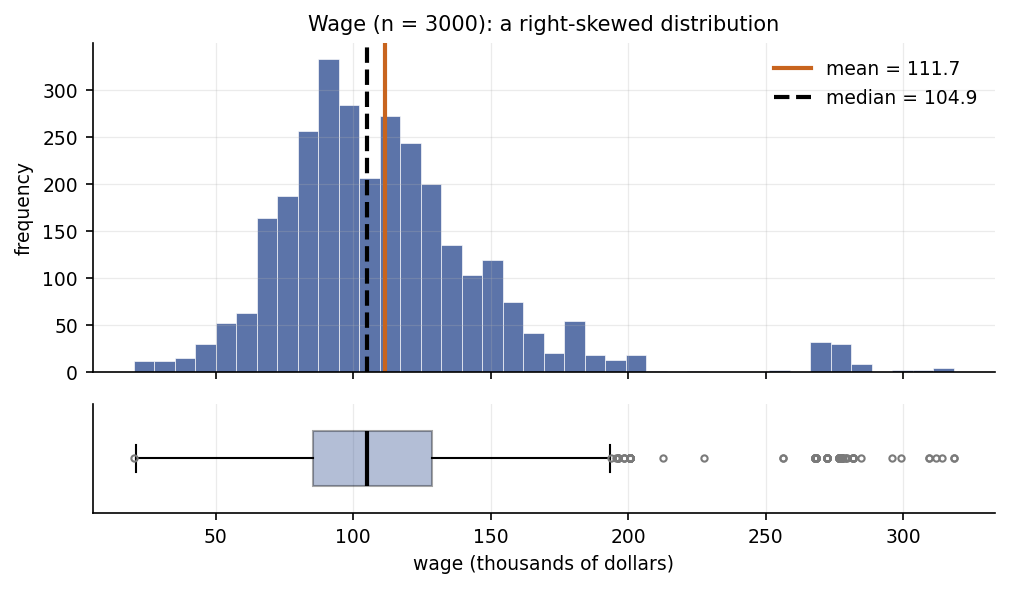
\includegraphics[width=0.72\textwidth,height=0.60\textheight,keepaspectratio]{ch00_center_spread.png}
  \end{center}
  \footnotesize
  \texttt{Wage} is right-skewed: a long upper tail pulls the mean
  ($111.7$) above the median ($104.9$). Rule of thumb: mean $>$ median
  suggests right skew, mean $<$ median left skew.
\end{frame}

\begin{frame}{Standardisation: the $z$-score}
  \begin{block}{Definition}
    \[
      z_i = \frac{x_i - \bar x}{s}
      \qquad\Longrightarrow\qquad
      \bar z = 0, \quad s_z = 1 .
    \]
  \end{block}
  \begin{takeaway}[Why you will meet this constantly]
    A $z$-score says ``how many standard deviations from the mean'', so it is
    unit-free and comparable across variables. It matters in:
    \begin{itemize}
      \item \textbf{Ch.\ 6} --- ridge and lasso penalise coefficients, so
            predictors \emph{must} be standardised first, or the penalty
            depends on whether you measured in euros or thousands of euros;
      \item \textbf{Ch.\ 2, 12} --- KNN and PCA use distances, which are
            dominated by whichever variable has the largest scale;
      \item \textbf{Ch.\ 10} --- neural networks train far better on
            standardised inputs.
    \end{itemize}
  \end{takeaway}
\end{frame}

\begin{frame}{Worked example: a seven-point sample by hand}
  \begin{numexample}[Seven observations computed by hand]
    \textbf{The data:} $2,\ 4,\ 4,\ 5,\ 7,\ 8,\ 12$ (so $n = 7$).

    \textbf{Centre.} $\sum x_i = 42$, so $\bar x = 42/7 = 6$. Sorted, the
    middle (4th) value is the median $=5$. The mode is $4$.

    \textbf{Spread.} Deviations $x_i - \bar x$: $-4,-2,-2,-1,1,2,6$; squares
    $16,4,4,1,1,4,36$, summing to $66$. Hence
    \[
      s^2 = \frac{66}{7-1} = 11, \qquad s = \sqrt{11} \approx 3.32 .
    \]
    \textbf{Quartiles.} Lower half $\{2,4,4\}$ gives $Q_1 = 4$; upper half
    $\{7,8,12\}$ gives $Q_3 = 8$; $\mathrm{IQR} = 4$. Fences:
    $4 - 6 = -2$ and $8 + 6 = 14$, so \emph{no} outliers --- $12$ is large but
    not flagged.

    \textbf{Shape.} $\bar x = 6 > 5 = $ median: mildly right-skewed, as the
    single large value $12$ suggests.
  \end{numexample}
\end{frame}

\begin{frame}{Exercise 0.2 --- Summaries and the effect of one outlier [Math]}
  \begin{exercise}
    Seven service times (minutes) were recorded:
    \[ 3,\quad 5,\quad 6,\quad 6,\quad 8,\quad 9,\quad 21 . \]
    \begin{enumerate}
      \item Compute the mean, the median and the mode.
      \item Compute $s^2$ and $s$. (Work with deviations from the mean.)
      \item Compute $Q_1$, $Q_3$ and the IQR, and apply the
            $1.5\times\mathrm{IQR}$ rule. Is $21$ an outlier?
      \item The $21$ was a typo for $12$. Recompute the mean and the median.
            Which moved more, and what general lesson does that illustrate?
    \end{enumerate}
  \end{exercise}
\end{frame}

\begin{frame}{Solution --- Exercise 0.2}
  \begin{solutionbox}
    \textbf{(1) Centre.} $\sum x_i = 3+5+6+6+8+9+21 = 58$, so
    $\bar x = 58/7 \approx 8.29$. The 4th of seven sorted values is the
    median $= 6$. The mode is $6$.

    \textbf{(2) Spread.} Deviations from $8.29$:
    $-5.29,-3.29,-2.29,-2.29,-0.29,0.71,12.71$; squares
    $27.9,10.8,5.2,5.2,0.1,0.5,161.6$, summing to $211.4$. Hence
    $s^2 = 211.4/6 \approx 35.2$ and $s \approx 5.94$ minutes.

    \textbf{(3) Quartiles.} Lower half $\{3,5,6\} \Rightarrow Q_1 = 5$; upper
    half $\{8,9,21\} \Rightarrow Q_3 = 9$; $\mathrm{IQR} = 4$. Upper fence
    $= 9 + 1.5(4) = 15 < 21$, so \textbf{yes}, $21$ is flagged as an outlier.
    (Flagged means \emph{investigate}, not \emph{delete}.)

    \textbf{(4) After the correction.} $\sum x_i = 49$, so $\bar x = 7$ ---
    it fell by $1.29$. The median is still $6$: unchanged. The mean is
    \emph{sensitive} to extreme values, the median is \emph{resistant}. This
    is exactly why skewed variables (income, waiting times, house prices)
    are reported with the median, and why a single mistyped value can move a
    least-squares fit --- squared errors magnify exactly this sensitivity
    (Chapter 3).
  \end{solutionbox}
\end{frame}


% ============================================================
\section{Describing two variables}
% ============================================================

\begin{frame}{Covariance: do two variables move together?}
  \begin{block}{Sample covariance}
    \[
      s_{xy} = \frac{1}{n-1}\sum_{i=1}^{n}(x_i - \bar x)(y_i - \bar y)
    \]
  \end{block}
  \begin{readme}[Reading the sign]
    Each term is positive when $x_i$ and $y_i$ are on the \emph{same} side of
    their means, negative otherwise. A positive sum means the variables tend
    to rise together; a negative sum means one rises as the other falls.
  \end{readme}
  \begin{takeaway}[The problem with covariance]
    Its size depends on units: measuring $x$ in cents rather than euros
    multiplies $s_{xy}$ by $100$, though nothing about the relationship
    changed. So we rescale it --- and get the correlation.
  \end{takeaway}
\end{frame}

\begin{frame}{Correlation: covariance made unit-free}
  \begin{block}{Pearson correlation}
    \[
      r = \frac{s_{xy}}{s_x s_y}
        = \frac{\sum_i (x_i-\bar x)(y_i-\bar y)}
               {\sqrt{\sum_i (x_i-\bar x)^2}\ \sqrt{\sum_i (y_i-\bar y)^2}},
      \qquad -1 \le r \le 1 .
    \]
  \end{block}
  \footnotesize
  \begin{tabular}{@{}ll@{}}
    \toprule
    \textbf{Value} & \textbf{Meaning} \\
    \midrule
    $r = +1$ / $-1$ & points lie exactly on an increasing / decreasing straight line \\
    $r \approx 0$ & no \emph{linear} association (there may still be a strong curved one) \\
    $|r|$ near $1$ & a tight linear pattern; near $0$, a diffuse cloud \\
    \bottomrule
  \end{tabular}
  \begin{takeaway}[Three warnings]
    $r$ measures \emph{linear} association only; it is not resistant to
    outliers; and it says nothing about \emph{causation} or about the
    \emph{slope} of the relationship.
  \end{takeaway}
\end{frame}

\begin{frame}{What $r$ sees --- and what it misses}
  \begin{center}
    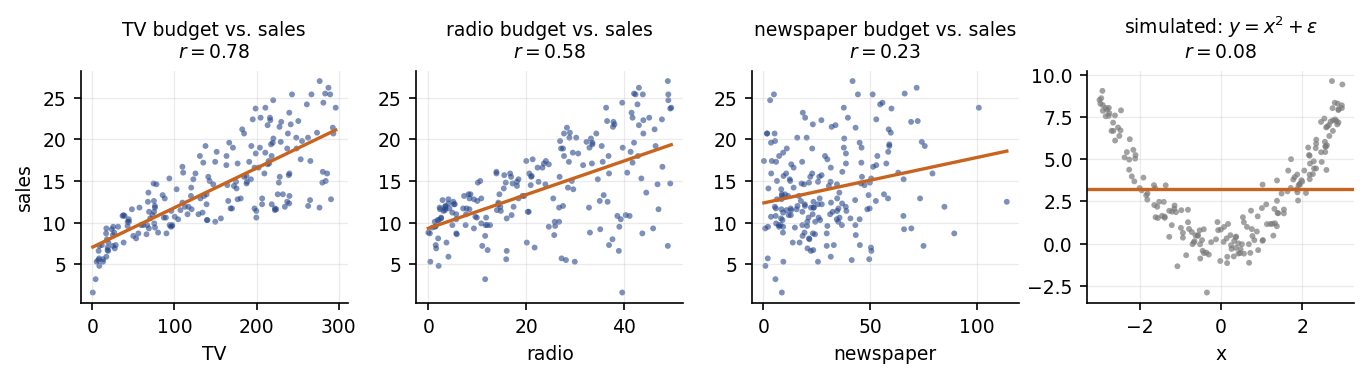
\includegraphics[width=0.98\textwidth,height=0.56\textheight,keepaspectratio]{ch00_correlation.png}
  \end{center}
  \footnotesize
  The first three panels use \texttt{Advertising}: TV spend tracks sales
  closely ($r = 0.78$), newspaper spend barely ($r = 0.23$). The fourth is
  simulated data with an obvious, \emph{strong} relationship
  $y = x^2 + \varepsilon$ --- and $r = 0.08$. \textbf{Always plot the data.}
\end{frame}

\begin{frame}{Correlation is not causation --- the two classic traps}
  \begin{readme}[Confounding]
    Ice-cream sales and drowning deaths correlate strongly. Neither causes
    the other: \emph{temperature} drives both. A variable that influences
    both $X$ and $Y$ is a \textbf{confounder}. Chapter 3 shows how adding it
    as a predictor can make a spurious effect disappear.
  \end{readme}
  \begin{readme}[Simpson's paradox]
    An association can \emph{reverse} once you condition on a group. A
    treatment can look worse overall yet be better in every subgroup, if the
    sicker patients were more likely to receive it. Aggregation can lie.
  \end{readme}
  \begin{takeaway}[The habit to build]
    Before believing any two-variable claim, ask: \emph{what third variable
    could produce this pattern?} This question is the entire reason
    multiple regression exists.
  \end{takeaway}
\end{frame}

\begin{frame}{Two categorical variables: the contingency table}
  \footnotesize
  A study of $200$ customers cross-tabulates a promotion against purchase:
  \begin{center}
  \begin{tabular}{@{}lccc@{}}
    \toprule
     & \textbf{Bought} & \textbf{Did not buy} & \textbf{Total} \\
    \midrule
    Received promotion & 45 & 55 & 100 \\
    No promotion       & 25 & 75 & 100 \\
    \midrule
    Total              & 70 & 130 & 200 \\
    \bottomrule
  \end{tabular}
  \end{center}
  \begin{itemize}
    \item \textbf{Row proportions} are what you compare: $45\%$ bought with the
          promotion vs.\ $25\%$ without.
    \item If the variables were independent, the expected count in a cell is
          $(\text{row total}\times\text{column total})/n$: here
          $100\times70/200 = 35$ for the top-left cell. Observed $45$ exceeds it.
    \item A $\chi^2$ test formalises whether that gap is bigger than chance.
  \end{itemize}
  \begin{takeaway}[Where this returns]
    This table is a \textbf{confusion matrix} in disguise. In Chapter 4 the
    rows become ``true class'' and the columns ``predicted class'', and the
    same proportions become sensitivity and specificity.
  \end{takeaway}
\end{frame}

\begin{frame}{Exercise 0.3 --- Covariance, correlation and a slope [Math]}
  \begin{exercise}
    Five stores report advertising spend $x$ (thousands of euros) and sales
    $y$ (thousands of units):
    \begin{center}\footnotesize
    \begin{tabular}{@{}lccccc@{}}
      \toprule
      $x$ & 1 & 2 & 3 & 4 & 5 \\
      $y$ & 2 & 4 & 5 & 4 & 10 \\
      \bottomrule
    \end{tabular}
    \end{center}
    \begin{enumerate}
      \item Compute $\bar x$ and $\bar y$.
      \item Compute $S_{xx} = \sum (x_i-\bar x)^2$,
            $S_{yy} = \sum (y_i-\bar y)^2$ and
            $S_{xy} = \sum (x_i-\bar x)(y_i-\bar y)$.
      \item Compute $r$. Describe the association in one sentence.
      \item The least-squares slope is $b_1 = S_{xy}/S_{xx}$. Compute it and
            state, in words and units, what it means.
      \item Why do $r$ and $b_1$ differ, even though both measure ``how $y$
            moves with $x$''?
    \end{enumerate}
  \end{exercise}
\end{frame}

\begin{frame}{Solution --- Exercise 0.3}
  \begin{solutionbox}
    \textbf{(1)} $\bar x = 15/5 = 3$, \quad $\bar y = 25/5 = 5$.

    \textbf{(2)} Deviations: $x_i - \bar x = -2,-1,0,1,2$ and
    $y_i - \bar y = -3,-1,0,-1,5$.
    \[
      S_{xx} = 4+1+0+1+4 = 10, \quad
      S_{yy} = 9+1+0+1+25 = 36, \quad
      S_{xy} = 6+1+0-1+10 = 16 .
    \]
    \textbf{(3)} $r = \dfrac{16}{\sqrt{10\cdot 36}} = \dfrac{16}{18.97}
    \approx 0.84$: a strong positive linear association --- stores that spend
    more on advertising tend to sell more.

    \textbf{(4)} $b_1 = 16/10 = 1.6$. \emph{One extra thousand euros of
    advertising is associated with $1.6$ thousand additional units sold},
    on average, in this sample. Note ``associated with'', not ``causes''.

    \textbf{(5)} They answer different questions. $r$ is unit-free and
    bounded in $[-1,1]$: it measures how \emph{tightly} the points hug a
    line. $b_1$ carries units (units per thousand euros): it measures how
    \emph{steeply} $y$ changes with $x$. Formally $b_1 = r\,s_y/s_x$ --- the
    same information, rescaled. A steep slope can be badly estimated
    (small $|r|$), and a tight relationship can have a nearly flat slope.
  \end{solutionbox}
\end{frame}


% ============================================================
\section{Probability essentials}
% ============================================================

\begin{frame}{The rules you actually need}
  \footnotesize
  \begin{block}{Basics}
    $0 \le P(A) \le 1$; \quad $P(\text{sure event}) = 1$; \quad
    $P(A^c) = 1 - P(A)$.
  \end{block}
  \begin{block}{Addition and multiplication}
    \[
      P(A \cup B) = P(A) + P(B) - P(A \cap B),
      \qquad
      P(A \cap B) = P(A \mid B)\,P(B).
    \]
  \end{block}
  \begin{block}{Conditional probability and independence}
    \[
      P(A \mid B) = \frac{P(A \cap B)}{P(B)} \quad (P(B) > 0);
      \qquad
      A \perp B \iff P(A \mid B) = P(A).
    \]
  \end{block}
  \begin{takeaway}[Conditioning is the whole game]
    Every classifier in this course estimates a conditional probability:
    $P(Y = \text{default} \mid X = \text{balance})$. ``Learning'' means
    turning data into a conditional probability you can act on.
  \end{takeaway}
\end{frame}

\begin{frame}{Bayes' theorem: reversing the conditioning}
  \begin{block}{The theorem}
    \[
      P(A \mid B) = \frac{P(B \mid A)\,P(A)}{P(B)},
      \qquad
      P(B) = P(B \mid A)P(A) + P(B \mid A^c)P(A^c).
    \]
  \end{block}
  \begin{readme}[What it is for]
    You know $P(\text{evidence} \mid \text{cause})$ --- how the test behaves
    for a sick person. You want $P(\text{cause} \mid \text{evidence})$ ---
    whether \emph{this} positive test means illness. Bayes' theorem
    converts one into the other, and the conversion depends on the
    \textbf{base rate} $P(A)$.
  \end{readme}
  \begin{takeaway}[Where it reappears]
    Chapter 4 is Bayes' theorem applied four times over: the Bayes
    classifier, LDA, QDA and naive Bayes all compute
    $P(Y=k \mid X=x)$ from $P(X = x\mid Y=k)$ and the prior $\pi_k = P(Y=k)$.
  \end{takeaway}
\end{frame}

\begin{frame}{Worked example: why a 95\% accurate test can mislead}
  \footnotesize
  \begin{numexample}[Screening for a rare condition]
    Prevalence $P(D) = 1\%$; sensitivity $P(+ \mid D) = 90\%$; specificity
    $P(- \mid D^c) = 95\%$, so $P(+ \mid D^c) = 5\%$. You test positive.
    \[
      P(+) = \underbrace{0.90 \times 0.01}_{\text{true positives } = 0.009}
           + \underbrace{0.05 \times 0.99}_{\text{false positives } = 0.0495}
           = 0.0585 .
    \]
    \[
      P(D \mid +) = \frac{0.009}{0.0585} \approx 0.154 .
    \]
    Only about \textbf{15\%}: the healthy group is $99$ times larger, so its
    $5\%$ false-positive rate produces five times more positives than the ill
    group does.
  \end{numexample}
  \begin{takeaway}[The lesson for Chapter 4]
    With rare events, high accuracy coexists with mostly-wrong positives ---
    which is why Chapter 4 reports sensitivity, specificity and ROC curves
    rather than one accuracy number.
  \end{takeaway}
\end{frame}

\begin{frame}{Random variables, expectation and variance}
  \begin{block}{Definitions (discrete case)}
    \[
      \mathrm{E}[X] = \sum_x x\,P(X=x),
      \qquad
      \mathrm{Var}(X) = \mathrm{E}\bigl[(X - \mathrm{E}[X])^2\bigr]
                      = \mathrm{E}[X^2] - (\mathrm{E}[X])^2 .
    \]
  \end{block}
  \begin{block}{Rules you will use constantly}
    \footnotesize
    \[
      \mathrm{E}[aX + b] = a\,\mathrm{E}[X] + b,
      \qquad
      \mathrm{Var}(aX + b) = a^2\,\mathrm{Var}(X),
    \]
    \[
      \mathrm{E}[X + Y] = \mathrm{E}[X] + \mathrm{E}[Y] \ \text{(always)},
      \qquad
      \mathrm{Var}(X + Y) = \mathrm{Var}(X) + \mathrm{Var}(Y)
      \ \text{\emph{only if} } X \perp Y .
    \]
  \end{block}
  \begin{takeaway}[Read the rules carefully]
    Expectation is linear \emph{without conditions}. Variance is not:
    adding a constant does not change spread ($b$ vanishes), scaling squares
    it ($a^2$), and variances add only under independence. The
    bias--variance decomposition in Chapter 2 is these rules applied to
    $\hat f(x)$.
  \end{takeaway}
\end{frame}

\begin{frame}{Exercise 0.4 --- Conditional probability and Bayes [Math]}
  \begin{exercise}
    A bank's fraud filter flags transactions. Historically $0.5\%$ of
    transactions are fraudulent. The filter flags $95\%$ of fraudulent
    transactions, and also flags $2\%$ of legitimate ones.
    \begin{enumerate}
      \item What proportion of \emph{all} transactions get flagged?
      \item A transaction is flagged. What is the probability that it is
            actually fraudulent?
      \item Out of $100{,}000$ transactions, fill in the four counts (fraud
            or not $\times$ flagged or not). Which cell dominates the flagged
            column?
      \item The bank wants $P(\text{fraud} \mid \text{flag})$ above $50\%$.
            Holding the $95\%$ detection rate fixed, what false-positive rate
            would be required? Comment on whether that is realistic.
    \end{enumerate}
  \end{exercise}
\end{frame}

\begin{frame}{Solution --- Exercise 0.4}
  \begin{solutionbox}
    \scriptsize
    \textbf{(1)} With $P(F) = 0.005$:
    \[
      P(\text{flag}) = 0.95(0.005) + 0.02(0.995)
                     = 0.00475 + 0.0199 = 0.02465 \approx 2.5\% .
    \]
    \textbf{(2)} $P(F \mid \text{flag}) = 0.00475/0.02465 \approx
    \textbf{19\%}$: four of five flags are false alarms, despite a $95\%$
    detection rate.

    \textbf{(3)} Per $100{,}000$ transactions:
    \begin{center}\scriptsize
    \begin{tabular}{@{}lccc@{}}
      \toprule
       & \textbf{Flagged} & \textbf{Not flagged} & \textbf{Total} \\
      \midrule
      Fraudulent & 475 & 25 & 500 \\
      Legitimate & 1{,}990 & 97{,}510 & 99{,}500 \\
      \midrule
      Total & 2{,}465 & 97{,}535 & 100{,}000 \\
      \bottomrule
    \end{tabular}
    \end{center}
    The $1{,}990$ false positives dominate: the legitimate group is $199$
    times larger, so even a small error rate on it swamps the true positives.

    \textbf{(4)} Require $0.00475/(0.00475 + f\cdot 0.995) \ge 0.5$, i.e.
    $f \le 0.0048$ --- a false-positive rate below \textbf{0.48\%}, four times
    stricter than today's $2\%$, and reachable only by flagging far less
    aggressively, which costs detection. That trade-off, drawn as a curve, is
    the ROC curve of Chapter 4.
  \end{solutionbox}
\end{frame}


% ============================================================
\section{Distributions you will meet}
% ============================================================

\begin{frame}{The discrete trio}
  \footnotesize
  \begin{block}{Bernoulli($\pi$) --- one yes/no trial}
    $P(X=1) = \pi$, $P(X=0) = 1-\pi$; $\mathrm{E}[X] = \pi$,
    $\mathrm{Var}(X) = \pi(1-\pi)$.
    \emph{Where:} the response in every classification problem
    (Ch.\ 4, 8, 10).
  \end{block}
  \begin{block}{Binomial($n,\pi$) --- number of successes in $n$ independent trials}
    $P(X=k) = \binom{n}{k}\pi^k(1-\pi)^{n-k}$; $\mathrm{E}[X] = n\pi$,
    $\mathrm{Var}(X) = n\pi(1-\pi)$.
    \emph{Where:} counting correct classifications; the bootstrap
    (Ch.\ 5).
  \end{block}
  \begin{block}{Poisson($\lambda$) --- counts per unit of time or space}
    $P(X=k) = e^{-\lambda}\lambda^k / k!$; $\mathrm{E}[X] = \mathrm{Var}(X) = \lambda$.
    \emph{Where:} Poisson regression on \texttt{Bikeshare} (Ch.\ 4).
  \end{block}
  \begin{takeaway}[Note the variance of a Bernoulli]
    $\pi(1-\pi)$ is largest at $\pi = 0.5$ and vanishes at $0$ or $1$: a
    near-certain event is nearly noiseless. This is why classification is
    hardest near the decision boundary.
  \end{takeaway}
\end{frame}

\begin{frame}{The normal distribution}
  \begin{block}{$X \sim N(\mu, \sigma^2)$}
    Symmetric and bell-shaped, fully determined by $\mu$ and $\sigma$.
    Standardising gives $Z = (X-\mu)/\sigma \sim N(0,1)$.
  \end{block}
  \begin{takeaway}[The 68--95--99.7 rule]
    About $68\%$ of the mass lies within $1\sigma$ of $\mu$, $95\%$ within
    $2\sigma$ (more precisely $1.96\sigma$), and $99.7\%$ within $3\sigma$.
    Memorising $1.96$ saves you a table lookup for the rest of the course.
  \end{takeaway}
  \begin{readme}[What is and is not assumed]
    Regression does \emph{not} require $X$ or $y$ to be normal. Normality
    is assumed for the \emph{errors} --- and even then mainly to justify
    $t$- and $F$-tests in small samples. With large $n$ the CLT does the
    work instead.
  \end{readme}
\end{frame}

\begin{frame}{Three distributions that come from the normal}
  \begin{center}
    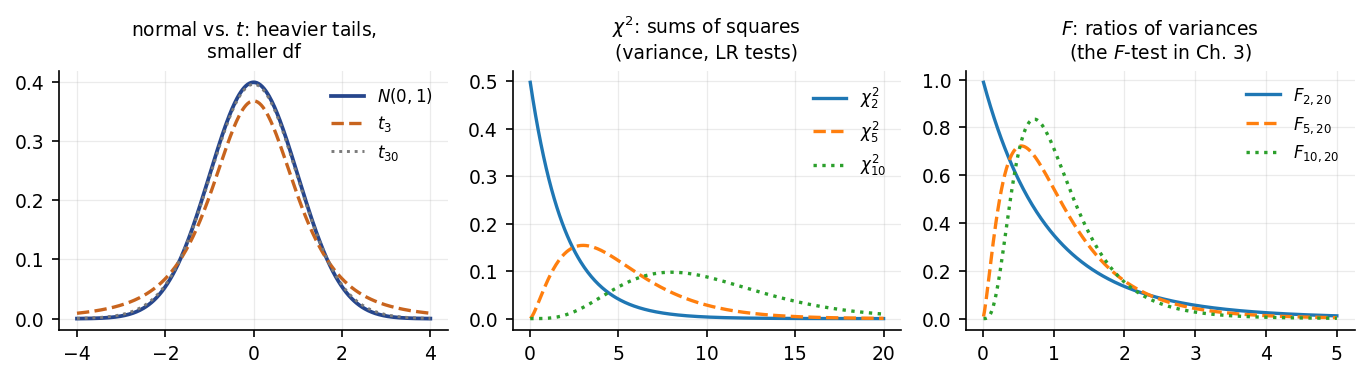
\includegraphics[width=0.98\textwidth,height=0.52\textheight,keepaspectratio]{ch00_reference_dists.png}
  \end{center}
  \footnotesize
  \begin{tabular}{@{}lll@{}}
    \toprule
    \textbf{Distribution} & \textbf{Arises as} & \textbf{Used for} \\
    \midrule
    $t_\nu$ & normal mean with $\sigma$ \emph{estimated} & $t$-tests, CIs on coefficients (Ch.\ 3) \\
    $\chi^2_\nu$ & sum of $\nu$ squared standard normals & variance, likelihood-ratio tests \\
    $F_{d_1,d_2}$ & ratio of two scaled $\chi^2$ & the $F$-test for several coefficients (Ch.\ 3) \\
    \bottomrule
  \end{tabular}
  \vspace{2pt}
  As the degrees of freedom grow, $t_\nu \to N(0,1)$: with $\nu > 30$ the
  difference is negligible, which is why large-sample rules of thumb use
  $1.96$.
\end{frame}

\begin{frame}{The central limit theorem}
  \begin{center}
    
\includegraphics[width=0.98\textwidth,height=0.50\textheight,keepaspectratio]{ch00_clt.png}
  \end{center}
  \begin{takeaway}[Statement]
    For a random sample of size $n$ from \emph{any} population with mean
    $\mu$ and finite variance $\sigma^2$,
    $\bar X \approx N\!\left(\mu, \sigma^2/n\right)$ for large $n$. The
    spread of $\bar X$ shrinks like $1/\sqrt{n}$ --- quadrupling the sample
    halves the uncertainty.
  \end{takeaway}
\end{frame}


% ============================================================
\section{Sampling, estimation and confidence intervals}
% ============================================================

\begin{frame}{Standard deviation vs.\ standard error}
  \footnotesize
  \begin{takeaway}[The distinction students most often blur]
    \begin{itemize}
      \item The \textbf{standard deviation} $s$ describes the spread of the
            \emph{data}; more data does not shrink it.
      \item The \textbf{standard error} $\mathrm{SE}(\bar x) = s/\sqrt{n}$
            describes the spread of an \emph{estimate} over repeated samples;
            more data \emph{does} shrink it.
    \end{itemize}
  \end{takeaway}
  \begin{numexample}[Numbers]
    Wages with $s = 40$ and $n = 100$: $\mathrm{SE}(\bar x) = 40/10 = 4$.
    With $n = 1600$: $\mathrm{SE} = 40/40 = 1$. The people are just as
    variable as before; our estimate of their average is four times more
    precise.
  \end{numexample}
  \begin{readme}[The habit]
    Report every estimate --- a coefficient, an error rate, a CV score ---
    \emph{with} its standard error. A number without an uncertainty is not a
    result.
  \end{readme}
\end{frame}

\begin{frame}{Confidence intervals}
  \begin{block}{The usual interval for a mean}
    \[
      \bar x \pm t_{n-1,\,0.975}\cdot \frac{s}{\sqrt{n}}
      \qquad\bigl(\approx \bar x \pm 1.96\,\mathrm{SE} \text{ for large } n\bigr).
    \]
  \end{block}
  \begin{center}
    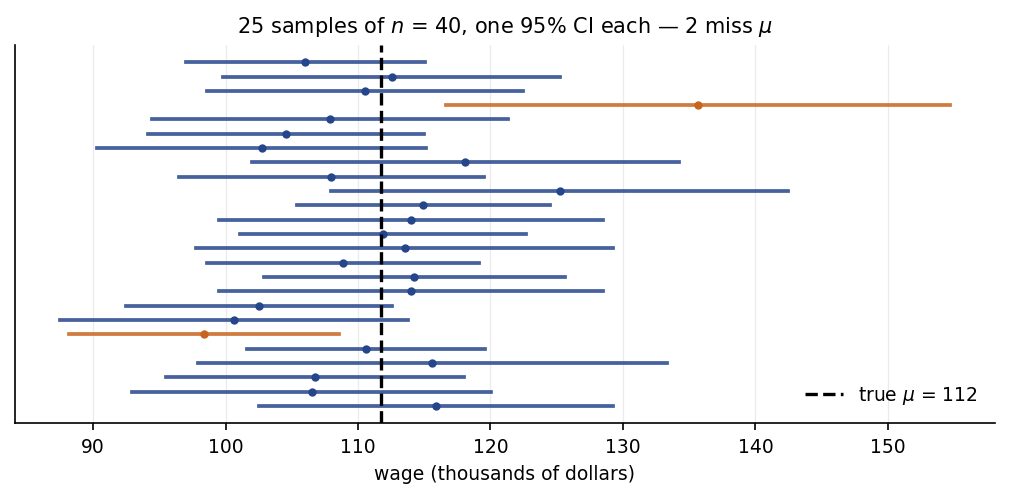
\includegraphics[width=0.66\textwidth,height=0.42\textheight,keepaspectratio]{ch00_ci_coverage.png}
  \end{center}
  \vspace{-2pt}
  \footnotesize
  Each horizontal bar is one 95\% CI from one sample. Two of the 25 miss the
  true $\mu$ --- which is exactly what ``95\%'' promises.
\end{frame}

\begin{frame}{What a confidence interval does and does not say}
  \footnotesize
  \begin{readme}[The correct reading]
    ``95\%'' is a property of the \emph{procedure}: repeat the whole
    sampling-and-computing exercise many times, and about 95\% of the
    intervals produced would contain the true parameter.
  \end{readme}
  \begin{alertblock}{Three wrong readings}
    \begin{enumerate}
      \item ``95\% probability that $\mu$ lies in \emph{this} interval.'' ---
            $\mu$ is fixed; this interval either contains it or not.
      \item ``95\% of the data lie in the interval.'' --- no: that is a
            \emph{prediction} interval, which is far wider.
      \item ``It contains 0, so the effect is zero.'' --- no: the data cannot
            rule zero out. Absence of evidence is not evidence of absence.
    \end{enumerate}
  \end{alertblock}
  \begin{takeaway}[Width tells you as much as position]
    Wide interval around a large estimate: ``possibly big --- we cannot tell''.
    Narrow interval around a small one: ``genuinely small''.
  \end{takeaway}
\end{frame}


% ============================================================
\section{Hypothesis testing}
% ============================================================

\begin{frame}{The logic of a test in five steps}
  \begin{enumerate}
    \item State $H_0$ (the sceptical default: ``no effect'', $\beta_j = 0$)
          and $H_1$.
    \item Choose $\alpha$, the false-positive rate you will tolerate
          (conventionally $0.05$).
    \item Compute a \textbf{test statistic}: the estimate, measured in
          standard errors, e.g.\ $t = (\hat\theta - \theta_0)/\mathrm{SE}(\hat\theta)$.
    \item Compute the \textbf{$p$-value}: the probability, \emph{if $H_0$ were
          true}, of a statistic at least this extreme.
    \item Reject $H_0$ if $p < \alpha$; otherwise fail to reject. Then report
          the \emph{estimate and its CI}, not just the verdict.
  \end{enumerate}
  \begin{takeaway}[The test statistic is a signal-to-noise ratio]
    $t$ asks: how large is the effect \emph{relative to how precisely we
    measured it}? Every $t$-value in every regression output in this course
    is exactly this ratio.
  \end{takeaway}
\end{frame}

\begin{frame}{Two ways to be wrong}
  \footnotesize
  \begin{center}
  \begin{tabular}{@{}lcc@{}}
    \toprule
     & \textbf{$H_0$ is true} & \textbf{$H_0$ is false} \\
    \midrule
    \textbf{Reject $H_0$} & Type I error (prob.\ $\alpha$) & correct (power $=1-\beta$) \\
    \textbf{Do not reject} & correct & Type II error (prob.\ $\beta$) \\
    \bottomrule
  \end{tabular}
  \end{center}
  \begin{itemize}
    \item Lowering $\alpha$ buys fewer false positives at the cost of more
          false negatives. There is no setting that avoids both.
    \item \textbf{Power} rises with the true effect size, with $n$, and with
          lower noise. Underpowered studies mostly produce misleading results.
  \end{itemize}
  \begin{takeaway}[The same table under different names]
    In Chapter 4 this becomes the confusion matrix (false positive / false
    negative); in Chapter 13 the columns are relabelled to define the family-wise
    error rate and the false discovery rate. It is one idea wearing three
    costumes.
  \end{takeaway}
\end{frame}

\begin{frame}{What a $p$-value is not}
  \begin{alertblock}{Four standard misreadings}
    \begin{enumerate}
      \item \emph{``$p = 0.03$ means a 3\% chance that $H_0$ is true.''} No:
            it is a probability computed \emph{assuming} $H_0$ --- it says
            nothing about $P(H_0 \mid \text{data})$.
      \item \emph{``$p > 0.05$ proves no effect.''} No: it may only mean the
            sample was too small to detect one.
      \item \emph{``$p = 0.001$ means a big effect.''} No: with huge $n$,
            trivial effects get tiny $p$-values. Significance $\neq$ importance.
      \item \emph{``I tested 20 things and one was significant at 5\%.''}
            Expected by chance alone --- see Chapter 13.
    \end{enumerate}
  \end{alertblock}
  \begin{takeaway}[The professional habit]
    Report the estimate, its confidence interval, and the $p$-value --- in
    that order of importance. Effect size first, uncertainty second, verdict
    last.
  \end{takeaway}
\end{frame}

\begin{frame}{Worked example: a one-sample $t$-test}
  \footnotesize
  \begin{numexample}[Has average handling time changed?]
    Historically a process took $\mu_0 = 100$ seconds. A sample of $n = 100$
    recent cases gives $\bar x = 103$ and $s = 15$.
    \[
      \mathrm{SE}(\bar x) = \frac{15}{\sqrt{100}} = 1.5,
      \qquad
      t = \frac{103 - 100}{1.5} = 2.00 \quad (\text{df} = 99).
    \]
    Two-sided $p \approx 0.048 < 0.05$: reject $H_0$ at the $5\%$ level.

    \textbf{The more useful statement.} The 95\% CI is
    $103 \pm 1.98(1.5) = [100.03,\ 105.97]$: the increase is somewhere
    between $0.03$ and $6$ seconds --- detectable, yet possibly far too small
    to matter operationally.
  \end{numexample}
  \begin{takeaway}[CI and test agree by construction]
    A two-sided test rejects at level $\alpha$ exactly when the
    $(1-\alpha)$ CI excludes the null value. The CI simply says more.
  \end{takeaway}
\end{frame}

\begin{frame}{Exercise 0.5 --- Reading an inference [Concept]}
  \begin{exercise}
    A colleague reports: ``We estimated the effect of a training programme on
    productivity. The estimate is $+2.4$ units with standard error $1.5$,
    giving $t = 1.6$ and $p = 0.11$. We conclude the programme has no
    effect.''
    \begin{enumerate}
      \item Compute the approximate 95\% confidence interval.
      \item Is the conclusion ``no effect'' justified? Answer using the
            interval.
      \item The team repeats the study with four times the sample size and
            obtains the same estimate $+2.4$. What is the new standard error
            (assuming the same variability), and the new $t$?
      \item In a second study of $40$ outcome variables, three came out
            significant at the $5\%$ level. Roughly how many would you expect
            by chance if none of the $40$ had any effect?
    \end{enumerate}
  \end{exercise}
\end{frame}

\begin{frame}{Solution --- Exercise 0.5}
  \begin{solutionbox}
    \textbf{(1)} $2.4 \pm 1.96(1.5) = 2.4 \pm 2.94 = [-0.54,\ 5.34]$.

    \textbf{(2)} \textbf{No.} The interval does contain $0$, so a zero effect
    cannot be ruled out --- but it also contains $+5.3$, a substantial
    benefit. The correct statement is ``this study cannot distinguish between
    no effect and a sizeable positive effect'': the data are
    \emph{inconclusive}, not evidence of absence. Failing to reject $H_0$ is
    never the same as accepting it.

    \textbf{(3)} The standard error scales as $1/\sqrt{n}$, so four times the
    data halves it: $\mathrm{SE} = 0.75$, and $t = 2.4/0.75 = 3.2$
    ($p \approx 0.001$). The new CI is $2.4 \pm 1.47 = [0.93,\ 3.87]$ ---
    same estimate, now clearly non-zero. \emph{Significance is as much about
    sample size as about the effect.}

    \textbf{(4)} With $40$ true nulls and $\alpha = 0.05$, we expect
    $40 \times 0.05 = \textbf{2}$ false positives, and $P(\text{at least
    one}) = 1 - 0.95^{40} \approx 0.87$. Three ``discoveries'' is therefore
    unremarkable. Correcting for this is the entire content of Chapter 13
    (Bonferroni, Holm, Benjamini--Hochberg).
  \end{solutionbox}
\end{frame}

\begin{frame}{Extended Exercise 0.1 --- From data to a defensible claim [Math]}
  \begin{longexercise}
    A retailer measures the basket value (euros) of $n = 64$ customers after
    a store redesign. The sample gives $\bar x = 48.5$ and $s = 12.0$. The
    pre-redesign average was $\mu_0 = 45.0$.
    \begin{enumerate}
      \item Compute $\mathrm{SE}(\bar x)$ and a 95\% confidence interval for
            the true post-redesign mean (use $1.96$).
      \item Test $H_0: \mu = 45$ against $H_1: \mu \ne 45$ at $\alpha = 0.05$.
            Report $t$ and your decision, and state how the CI would have
            told you the same thing.
      \item Management says an increase is worth acting on only if it exceeds
            \euro 5. Does the evidence support acting? Answer using the
            interval, not the $p$-value.
      \item How large would $n$ have to be for the CI half-width to shrink to
            \euro 1.00 (same $s$)?
      \item The redesign coincided with a marketing campaign. What does that
            do to the causal interpretation, and what design would fix it?
    \end{enumerate}
  \end{longexercise}
\end{frame}

\begin{frame}{Solution --- Extended Exercise 0.1 (1/2)}
  \begin{solutionbox}
    \textbf{(1) Standard error and interval.}
    \[
      \mathrm{SE}(\bar x) = \frac{s}{\sqrt n} = \frac{12}{\sqrt{64}}
      = \frac{12}{8} = 1.5 .
    \]
    \[
      \text{95\% CI} = 48.5 \pm 1.96(1.5) = 48.5 \pm 2.94
      = [\,45.56,\ 51.44\,] .
    \]

    \textbf{(2) The test.}
    \[
      t = \frac{\bar x - \mu_0}{\mathrm{SE}} = \frac{48.5 - 45.0}{1.5}
        = \frac{3.5}{1.5} = 2.33 \quad (\text{df} = 63).
    \]
    Two-sided $p \approx 0.023 < 0.05$, so we reject $H_0$: the mean basket
    value differs from \euro 45. The CI says the same thing without a
    separate calculation --- it excludes $45$. This equivalence is exact for
    a two-sided test at the matching level.
  \end{solutionbox}
\end{frame}

\begin{frame}{Solution --- Extended Exercise 0.1 (2/2)}
  \begin{solutionbox}
    \textbf{(3) The decision that management actually asked about.}
    The relevant question is not ``is the increase non-zero'' but ``is it
    above \euro 5''. The increase is estimated at
    $48.5 - 45.0 = \text{\euro} 3.50$, with CI
    $[45.56, 51.44] - 45 = [\,0.56,\ 6.44\,]$. The interval straddles $5$:
    the data are consistent with an increase of \euro 1 and with one of
    \euro 6. So the evidence does \emph{not} support acting --- and note that
    the $p$-value alone ($0.023$, ``significant'') would have suggested the
    opposite. \emph{Statistical significance answered the wrong question.}

    \textbf{(4) Required sample size.} Half-width
    $1.96 \cdot 12/\sqrt{n} \le 1.00$ requires
    $\sqrt n \ge 1.96 \cdot 12 = 23.52$, so $n \ge 553.2$, i.e.\
    $n = \textbf{554}$. Nearly nine times the data for a threefold gain in
    precision --- the $1/\sqrt{n}$ law is unforgiving, and it is the same law
    that makes learning curves flatten in Chapter 2.

    \textbf{(5) Causality.} The campaign is a \textbf{confounder}: the
    redesign and the campaign changed together, so their effects cannot be
    separated from these data --- they are \emph{confounded} in the technical
    sense. Fixes, in descending order of quality: randomise stores to
    redesign / no redesign while running the campaign everywhere; or use
    control stores with the campaign but no redesign (difference-in-differences);
    or, weakest, adjust for campaign exposure in a regression --- which only
    works for confounders you thought to measure.
  \end{solutionbox}
\end{frame}


% ============================================================
\section{Simple linear regression: the bridge}
% ============================================================

\begin{frame}{The model and the criterion}
  \begin{block}{The model}
    \[
      y_i = \beta_0 + \beta_1 x_i + \varepsilon_i,
      \qquad \mathrm{E}[\varepsilon_i] = 0 .
    \]
  \end{block}
  \begin{block}{Least squares}
    Choose $b_0, b_1$ minimising the residual sum of squares
    \[
      \mathrm{RSS}(b_0,b_1) = \sum_{i=1}^{n}\bigl(y_i - b_0 - b_1 x_i\bigr)^2 ,
      \qquad
      b_1 = \frac{S_{xy}}{S_{xx}}, \quad b_0 = \bar y - b_1 \bar x .
    \]
  \end{block}
  \begin{takeaway}[Two things to notice now]
    (i) The fitted line always passes through $(\bar x, \bar y)$.
    (ii) Squared errors are chosen for tractability, not sanctity --- they
    make the algebra closed-form, and they make outliers expensive.
  \end{takeaway}
\end{frame}

\begin{frame}{Fitted values, residuals, and $R^2$}
  \begin{center}
    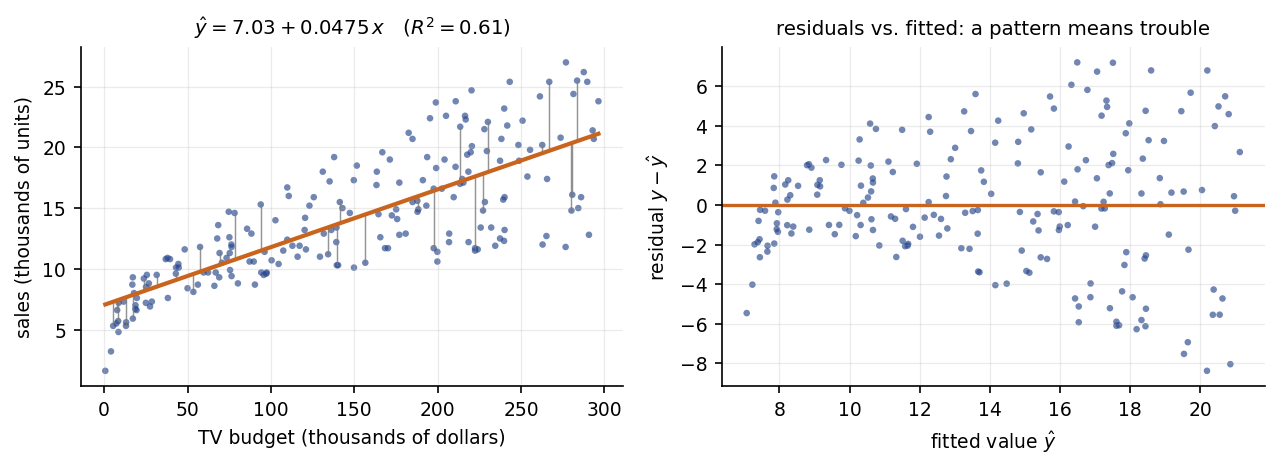
\includegraphics[width=0.92\textwidth,height=0.50\textheight,keepaspectratio]{ch00_slr.png}
  \end{center}
  \footnotesize
  Left: the fit on \texttt{Advertising}; the grey segments are the residuals
  $e_i = y_i - \hat y_i$ that least squares squares and adds up. Right: a
  residual plot --- structure here (curvature, a funnel) means the model is
  missing something. Both plots return in Chapter 3.
\end{frame}

\begin{frame}{Decomposing the variation}
  \footnotesize
  \begin{block}{The three sums of squares}
    \[
      \underbrace{\sum_i (y_i - \bar y)^2}_{\mathrm{TSS}}
      = \underbrace{\sum_i (\hat y_i - \bar y)^2}_{\text{explained}}
      + \underbrace{\sum_i (y_i - \hat y_i)^2}_{\mathrm{RSS}},
      \qquad
      R^2 = 1 - \frac{\mathrm{RSS}}{\mathrm{TSS}} .
    \]
  \end{block}
  \begin{readme}[How to read $R^2$]
    The fraction of the variation in $y$ that the model accounts for.
    $R^2 = 0.61$ means ``61\% of the variability in sales is accounted for by
    TV spend''. In simple regression $R^2 = r^2$ exactly.
  \end{readme}
  \begin{alertblock}{Do not over-read it}
    A high $R^2$ does not make a model correct, useful or causal, and a low
    one does not make it worthless. Adding any predictor never decreases
    $R^2$ --- which is why Chapter 6 needs adjusted $R^2$, $C_p$, AIC, BIC and
    cross-validation.
  \end{alertblock}
\end{frame}

\begin{frame}{Extended Exercise 0.2 --- Regression by hand, end to end [Math]}
  \begin{longexercise}
    Four branches report weekly advertising spend $x$ (\euro 000s) and sales
    $y$ (\euro 000s):
    \begin{center}\footnotesize
    \begin{tabular}{@{}lcccc@{}}
      \toprule
      $x$ & 2 & 4 & 6 & 8 \\
      $y$ & 5 & 8 & 12 & 15 \\
      \bottomrule
    \end{tabular}
    \end{center}
    \begin{enumerate}
      \item Compute $\bar x$, $\bar y$, $S_{xx}$, $S_{xy}$ and $S_{yy}$.
      \item Compute $b_1$ and $b_0$, and write out the fitted line.
      \item Compute the four fitted values and residuals. Verify that the
            residuals sum to (approximately) zero, and explain why they must.
      \item Compute RSS, TSS and $R^2$. Confirm $R^2 = r^2$.
      \item Interpret $b_0$ and $b_1$ in words \emph{with units}. Is the
            interpretation of $b_0$ trustworthy here?
      \item Predict sales at $x = 5$ and at $x = 40$. Which prediction would
            you defend, and why?
    \end{enumerate}
  \end{longexercise}
\end{frame}

\begin{frame}{Solution --- Extended Exercise 0.2 (1/2)}
  \begin{solutionbox}
    \textbf{(1) Sums.} $\bar x = 20/4 = 5$, $\bar y = 40/4 = 10$.
    Deviations $x_i - \bar x = -3,-1,1,3$ and $y_i - \bar y = -5,-2,2,5$.
    \[
      S_{xx} = 9+1+1+9 = 20, \quad
      S_{xy} = 15+2+2+15 = 34, \quad
      S_{yy} = 25+4+4+25 = 58 .
    \]
    \textbf{(2) Coefficients.}
    \[
      b_1 = \frac{34}{20} = 1.7,
      \qquad
      b_0 = 10 - 1.7(5) = 1.5,
      \qquad
      \hat y = 1.5 + 1.7x .
    \]
    \textbf{(3) Fitted values and residuals.}
    \begin{center}\scriptsize
    \begin{tabular}{@{}lcccc@{}}
      \toprule
      $x_i$ & 2 & 4 & 6 & 8 \\
      $\hat y_i = 1.5+1.7x_i$ & 4.9 & 8.3 & 11.7 & 15.1 \\
      $e_i = y_i - \hat y_i$ & $+0.1$ & $-0.3$ & $+0.3$ & $-0.1$ \\
      \bottomrule
    \end{tabular}
    \end{center}
    The residuals sum to $0$. This is forced by the first normal equation:
    setting $\partial \mathrm{RSS}/\partial b_0 = 0$ gives
    $\sum_i e_i = 0$ exactly. It is a property of the \emph{fitting method},
    not evidence that the model is right.
  \end{solutionbox}
\end{frame}

\begin{frame}{Solution --- Extended Exercise 0.2 (2/2)}
  \begin{solutionbox}
    \textbf{(4) Fit quality.}
    $\mathrm{RSS} = 0.1^2+0.3^2+0.3^2+0.1^2 = 0.01+0.09+0.09+0.01 = 0.20$,
    and $\mathrm{TSS} = S_{yy} = 58$. So
    \[
      R^2 = 1 - \frac{0.20}{58} = 0.99655 .
    \]
    Check: $r = S_{xy}/\sqrt{S_{xx}S_{yy}} = 34/\sqrt{20 \cdot 58}
    = 34/34.06 = 0.99827$, and $r^2 = 0.99655$. \checkmark

    \textbf{(5) Interpretation.} $b_1 = 1.7$: each additional
    \euro 1{,}000 of weekly advertising is associated with \euro 1{,}700 more
    weekly sales, on average. $b_0 = 1.5$: predicted sales of \euro 1{,}500
    at \emph{zero} advertising. Treat $b_0$ with care --- $x = 0$ is outside
    the observed range $[2,8]$, so it is an extrapolation, and here it is
    merely the intercept that makes the line fit, not a meaningful
    ``baseline''.

    \textbf{(6) Predictions.} At $x = 5$: $\hat y = 1.5 + 8.5 = 10.0$ ---
    defensible, since $5$ sits inside the observed range (interpolation). At
    $x = 40$: $\hat y = 1.5 + 68 = 69.5$ --- \emph{not} defensible: it is
    five times beyond the largest observed spend, where linearity is
    untested and diminishing returns are likely. Never extrapolate a fitted
    model far outside the data it was estimated from; with $n = 4$ the fit
    is fragile in any case.
  \end{solutionbox}
\end{frame}


% ============================================================
\section{Linear algebra you will need}
% ============================================================

\begin{frame}{Vectors and matrices: the minimum}
  \footnotesize
  \begin{block}{Objects}
    A \textbf{vector} $\mathbf{a} \in \mathbb{R}^p$ is a column of $p$
    numbers; an $m \times n$ \textbf{matrix} has $m$ rows and $n$ columns;
    $\mathbf{A}^\top$ swaps them.
  \end{block}
  \begin{block}{Multiplication --- the only rule you must remember}
    $(m \times n)\cdot(n \times k) = (m \times k)$: the \emph{inner}
    dimensions must match and they disappear. Entry $(i,j)$ of the product is
    the dot product of row $i$ of the first and column $j$ of the second.
  \end{block}
  \begin{block}{Special cases}
    Dot product $\mathbf{a}^\top\mathbf{b} = \sum_j a_j b_j$ (a scalar);
    identity $\mathbf{I}$ with $\mathbf{A}\mathbf{I} = \mathbf{A}$;
    inverse $\mathbf{A}^{-1}$ with $\mathbf{A}^{-1}\mathbf{A} = \mathbf{I}$
    (exists only if $\mathbf{A}$ is square and non-singular).
  \end{block}
  \begin{takeaway}[Dimension checking is free error-detection]
    If $\mathbf{X}$ is $n \times p$, then $\mathbf{X}^\top\mathbf{X}$ is
    $p \times p$ and $\mathbf{X}^\top\mathbf{y}$ is $p \times 1$. Any formula
    whose dimensions do not line up is wrong --- no algebra needed.
  \end{takeaway}
\end{frame}

\begin{frame}{Why this course speaks matrix}
  \begin{block}{Regression in one line}
    With a column of ones in $\mathbf{X}$, the least-squares estimator is
    \[
      \hat{\boldsymbol\beta}
      = (\mathbf{X}^\top\mathbf{X})^{-1}\mathbf{X}^\top\mathbf{y},
      \qquad
      \hat{\mathbf{y}} = \mathbf{X}\hat{\boldsymbol\beta}.
    \]
  \end{block}
  \begin{readme}[Read it as a recipe]
    $\mathbf{X}^\top\mathbf{y}$ collects how each predictor covaries with the
    response; $\mathbf{X}^\top\mathbf{X}$ records how they covary with
    \emph{each other}; inverting it divides out that shared information ---
    which is what ``holding the others constant'' means algebraically.
  \end{readme}
  \begin{alertblock}{When the inverse fails}
    If two predictors are perfectly correlated, or $p > n$, then
    $\mathbf{X}^\top\mathbf{X}$ is singular and $\hat{\boldsymbol\beta}$ does
    not exist. Ridge regression inverts
    $\mathbf{X}^\top\mathbf{X} + \lambda\mathbf{I}$ instead (Ch.\ 6).
  \end{alertblock}
\end{frame}

\begin{frame}{Norms, distances and eigenvectors --- where they show up}
  \footnotesize
  \begin{block}{Norms}
    \[
      \|\boldsymbol\beta\|_2^2 = \sum_j \beta_j^2 \quad(\ell_2),
      \qquad
      \|\boldsymbol\beta\|_1 = \sum_j |\beta_j| \quad(\ell_1).
    \]
    \emph{Where:} ridge penalises $\|\boldsymbol\beta\|_2^2$ and shrinks
    coefficients smoothly; lasso penalises $\|\boldsymbol\beta\|_1$ and sets
    some to exactly zero (Ch.\ 6). The difference between a round and a
    pointed constraint region is the whole story.
  \end{block}
  \begin{block}{Euclidean distance}
    $d(\mathbf{a},\mathbf{b}) = \sqrt{\sum_j (a_j-b_j)^2}$.
    \emph{Where:} KNN (Ch.\ 2, 4) and clustering (Ch.\ 12) are built on it ---
    and it is why unstandardised variables wreck both.
  \end{block}
  \begin{block}{Eigenvectors and eigenvalues}
    $\mathbf{A}\mathbf{v} = \lambda\mathbf{v}$: directions the matrix only
    stretches. \emph{Where:} principal components (Ch.\ 6, 12) are the
    eigenvectors of the covariance matrix --- the directions of greatest
    variance in the data.
  \end{block}
\end{frame}

\begin{frame}{Exercise 0.6 --- Matrix mechanics [Math]}
  \begin{exercise}
    Let
    \[
      \mathbf{X} = \begin{pmatrix} 1 & 1 \\ 1 & 2 \\ 1 & 3 \end{pmatrix},
      \qquad
      \mathbf{y} = \begin{pmatrix} 2 \\ 3 \\ 5 \end{pmatrix}.
    \]
    \begin{enumerate}
      \item State the dimensions of $\mathbf{X}^\top$,
            $\mathbf{X}^\top\mathbf{X}$ and $\mathbf{X}^\top\mathbf{y}$
            \emph{before} computing anything.
      \item Compute $\mathbf{X}^\top\mathbf{X}$ and
            $\mathbf{X}^\top\mathbf{y}$.
      \item Invert $\mathbf{X}^\top\mathbf{X}$, using
            $\begin{pmatrix} a & b \\ c & d\end{pmatrix}^{-1}
             = \frac{1}{ad-bc}\begin{pmatrix} d & -b \\ -c & a\end{pmatrix}$.
      \item Compute
            $\hat{\boldsymbol\beta}
             = (\mathbf{X}^\top\mathbf{X})^{-1}\mathbf{X}^\top\mathbf{y}$,
            and check the slope against $b_1 = S_{xy}/S_{xx}$.
      \item What would go wrong if a third column equal to twice the second
            were added to $\mathbf{X}$?
    \end{enumerate}
  \end{exercise}
\end{frame}

\begin{frame}{Solution --- Exercise 0.6}
  \begin{solutionbox}
    \textbf{(1)} $\mathbf{X}$ is $3\times2$, so $\mathbf{X}^\top$ is
    $2\times3$, $\mathbf{X}^\top\mathbf{X}$ is $2\times2$ and
    $\mathbf{X}^\top\mathbf{y}$ is $2\times1$; hence
    $\hat{\boldsymbol\beta}$ is $2\times1$ --- an intercept and a slope.

    \textbf{(2)}
    \[
      \mathbf{X}^\top\mathbf{X}
      = \begin{pmatrix} 3 & 6 \\ 6 & 14 \end{pmatrix},
      \qquad
      \mathbf{X}^\top\mathbf{y}
      = \begin{pmatrix} 2+3+5 \\ 2+6+15 \end{pmatrix}
      = \begin{pmatrix} 10 \\ 23 \end{pmatrix}.
    \]
    \textbf{(3)} $\det = 3(14) - 6(6) = 42 - 36 = 6$, so
    $(\mathbf{X}^\top\mathbf{X})^{-1}
      = \frac{1}{6}\begin{pmatrix} 14 & -6 \\ -6 & 3\end{pmatrix}$.

    \textbf{(4)}
    \[
      \hat{\boldsymbol\beta} = \frac{1}{6}
      \begin{pmatrix} 14 & -6 \\ -6 & 3\end{pmatrix}
      \begin{pmatrix} 10 \\ 23 \end{pmatrix}
      = \frac{1}{6}\begin{pmatrix} 140-138 \\ -60+69 \end{pmatrix}
      = \frac{1}{6}\begin{pmatrix} 2 \\ 9 \end{pmatrix}
      = \begin{pmatrix} 0.333 \\ 1.5 \end{pmatrix}.
    \]
    Check: $\bar x = 2$, $\bar y = 10/3$, $S_{xx} = 2$, $S_{xy} = 3$, so
    $b_1 = 1.5$ \checkmark and $b_0 = 10/3 - 3 = 1/3$ \checkmark.

    \textbf{(5)} Perfect collinearity: $\mathbf{X}^\top\mathbf{X}$ becomes
    singular ($\det = 0$), the inverse does not exist, and infinitely many
    coefficient vectors give an identical fit. Software reports a ``singular
    matrix'' or silently drops a column.
  \end{solutionbox}
\end{frame}


% ============================================================
\section{Calculus and optimisation}
% ============================================================

\begin{frame}{Derivatives: the three facts that matter}
  \footnotesize
  \begin{block}{Rules}
    \[
      \frac{d}{dx}x^k = kx^{k-1},
      \qquad
      \frac{d}{dx}e^x = e^x,
      \qquad
      \frac{d}{dx}\log x = \frac1x,
      \qquad
      \frac{d}{dx}f(g(x)) = f'(g(x))\,g'(x).
    \]
  \end{block}
  \begin{block}{What a derivative means here}
    The slope of the function: how much the output changes per unit change
    in the input. At a minimum, the slope is zero --- which is how every
    estimator in this course is derived.
  \end{block}
  \begin{block}{Partial derivatives and the gradient}
    With several inputs, differentiate with respect to one at a time,
    holding the others fixed. Stacking them gives the gradient
    \[
      \nabla f(\boldsymbol\beta)
      = \Bigl(\tfrac{\partial f}{\partial \beta_1}, \dots,
              \tfrac{\partial f}{\partial \beta_p}\Bigr)^{\!\top},
    \]
    which points in the direction of \emph{steepest increase}.
  \end{block}
\end{frame}

\begin{frame}{Minimising a loss: the pattern behind every method}
  \begin{numexample}[Deriving the sample mean]
    Minimise $L(c) = \sum_i (x_i - c)^2$ over $c$:
    \[
      \frac{dL}{dc} = -2\sum_i (x_i - c) = 0
      \;\Longrightarrow\;
      \sum_i x_i = nc
      \;\Longrightarrow\;
      c = \bar x .
    \]
    So the sample mean is not a convention --- it is \emph{the} minimiser of
    squared error. (Minimising $\sum_i |x_i - c|$ instead gives the median.)
  \end{numexample}
  \begin{takeaway}[The recurring recipe]
    \textbf{1.} Write a loss measuring misfit. \textbf{2.} Differentiate.
    \textbf{3.} Set to zero and solve --- or, when no closed form exists,
    walk downhill. Least squares, logistic regression, splines, boosting and
    neural networks are all this recipe with different losses.
  \end{takeaway}
\end{frame}

\begin{frame}{Gradient descent: when there is no closed form}
  \begin{block}{The update}
    \[
      \boldsymbol\beta^{(t+1)}
      = \boldsymbol\beta^{(t)} - \alpha\,\nabla L\bigl(\boldsymbol\beta^{(t)}\bigr),
      \qquad \alpha > 0 \text{ the learning rate}.
    \]
  \end{block}
  \begin{readme}[The picture]
    Stand on a hillside in fog. The gradient points uphill, so step the
    opposite way, and repeat. $\alpha$ too small $\Rightarrow$ crawling;
    $\alpha$ too large $\Rightarrow$ overshooting and divergence. Choosing
    it well is a recurring practical theme of Chapter 10.
  \end{readme}
  \begin{takeaway}[Convexity decides whether this is safe]
    For a convex loss (least squares, logistic regression) every local
    minimum is global, so descent finds the answer. Neural networks are
    \emph{not} convex --- which is why initialisation, learning-rate
    schedules and early stopping matter so much in Chapter 10.
  \end{takeaway}
\end{frame}

\begin{frame}{Extended Exercise 0.3 --- Normal equations and one descent step [Integrative]}
  \begin{longexercise}
    Use the data of Exercise 0.6:
    $(x,y) = (1,2), (2,3), (3,5)$, model $y = \beta_0 + \beta_1 x$, and
    loss $L(\boldsymbol\beta) = \sum_i (y_i - \beta_0 - \beta_1 x_i)^2$.
    \begin{enumerate}
      \item Write $L$ out explicitly for the three observations.
      \item Derive $\partial L/\partial\beta_0$ and
            $\partial L/\partial\beta_1$, and show that setting both to zero
            gives the normal equations
            $\mathbf{X}^\top\mathbf{X}\boldsymbol\beta = \mathbf{X}^\top\mathbf{y}$.
      \item Starting from $\boldsymbol\beta^{(0)} = (0,0)^\top$, compute the
            gradient and take one gradient-descent step with $\alpha = 0.01$.
      \item Compute $L$ at $\boldsymbol\beta^{(0)}$, at
            $\boldsymbol\beta^{(1)}$, and at the exact solution
            $(1/3,\ 3/2)^\top$. Did the step help?
      \item What happens with $\alpha = 1$? Compute
            $\boldsymbol\beta^{(1)}$ and comment.
    \end{enumerate}
  \end{longexercise}
\end{frame}

\begin{frame}{Solution --- Extended Exercise 0.3 (1/2)}
  \begin{solutionbox}
    \scriptsize
    \textbf{(1) The loss.}
    \[
      L(\beta_0,\beta_1) = (2-\beta_0-\beta_1)^2 + (3-\beta_0-2\beta_1)^2
                         + (5-\beta_0-3\beta_1)^2 .
    \]
    \textbf{(2) Partial derivatives.} With $e_i = y_i-\beta_0-\beta_1x_i$,
    \[
      \frac{\partial L}{\partial \beta_0} = -2\sum_i e_i,
      \qquad
      \frac{\partial L}{\partial \beta_1} = -2\sum_i x_i e_i .
    \]
    Setting both to zero gives $\sum_i e_i = 0$ and $\sum_i x_i e_i = 0$, i.e.
    $3\beta_0 + 6\beta_1 = 10$ and $6\beta_0 + 14\beta_1 = 23$ --- exactly
    $\mathbf{X}^\top\mathbf{X}\boldsymbol\beta = \mathbf{X}^\top\mathbf{y}$
    with the matrices of Exercise 0.6, so
    $\boldsymbol\beta = (1/3,\ 3/2)^\top$ as before. \emph{The normal
    equations are ``derivative $=0$'' in matrix form.}

    \textbf{(3) One step.} At $(0,0)^\top$ the residuals are $e = (2,3,5)$:
    \[
      \nabla L = -2\bigl(\textstyle\sum_i e_i,\ \sum_i x_i e_i\bigr)^\top
               = -2(10,\ 23)^\top = (-20,\ -46)^\top ,
    \]
    \[
      \boldsymbol\beta^{(1)} = (0,0)^\top - 0.01(-20,-46)^\top
                             = (0.20,\ 0.46)^\top .
    \]
    The step moves \emph{towards} $(0.33, 1.50)$, as it should.
  \end{solutionbox}
\end{frame}

\begin{frame}{Solution --- Extended Exercise 0.3 (2/2)}
  \begin{solutionbox}
    \textbf{(4) Did it help?}
    \[
      L(0,0) = 2^2+3^2+5^2 = 38 .
    \]
    At $\boldsymbol\beta^{(1)} = (0.20, 0.46)$ the fitted values are
    $0.66, 1.12, 1.58$, so the residuals are $1.34, 1.88, 3.42$ and
    \[
      L(\boldsymbol\beta^{(1)}) = 1.796 + 3.534 + 11.696 = 17.03 .
    \]
    At the exact solution the residuals are $1/6, -1/3, 1/6$, so
    $L = 1/6 \approx 0.167$. One step cut the loss from $38$ to $17$ --- a big
    improvement, still far from the optimum: descent needs many iterations,
    which is why a closed form is preferred whenever one exists.

    \textbf{(5) Too large a learning rate.} With $\alpha = 1$,
    \[
      \boldsymbol\beta^{(1)} = (0,0)^\top - 1\cdot(-20,-46)^\top = (20,\ 46)^\top .
    \]
    Fitted values are $66, 112, 158$ against $y = (2,3,5)$: the loss explodes
    to about $4.1\times10^{4}$, far worse than the starting $38$, and the next
    step is larger still --- \textbf{divergence}. The step size must respect
    the curvature of the loss, so in practice one standardises the predictors
    and tunes $\alpha$: the workflow of Chapter 10.
  \end{solutionbox}
\end{frame}


% ============================================================
\section{The Python toolkit}
% ============================================================

\begin{frame}[fragile]{\texttt{numpy}: arrays and vectorised arithmetic}
\begin{lstlisting}
import numpy as np

x = np.array([2, 4, 4, 5, 7, 8, 12])   # a 1-D array
x.mean(), np.median(x), x.std(ddof=1)  # 6.0, 5.0, 3.317

z = (x - x.mean()) / x.std(ddof=1)     # vectorised: no loop needed
A = np.array([[1, 1], [1, 2], [1, 3]]) # a 3x2 matrix
A.T @ A                                # matrix product: 2x2
\end{lstlisting}
  \begin{alertblock}{The one trap}
    \texttt{np.std()} divides by $n$ by default, not $n-1$. Pass
    \texttt{ddof=1} for the \emph{sample} standard deviation. (\texttt{pandas}
    uses $n-1$ by default --- the two libraries disagree, so state what you
    mean.)
  \end{alertblock}
\end{frame}

\begin{frame}[fragile]{\texttt{pandas}: the data frame is your data set}
\begin{lstlisting}
import pandas as pd

df = pd.read_csv("Wage.csv", index_col=0)
df.shape          # (3000, 11) -- that's (n, p)
df.head()         # first rows
df.describe()     # count, mean, std, min, quartiles, max
df["wage"].median()
df["education"].value_counts()          # categorical: counts
df.groupby("education")["wage"].mean()  # a summary per group
df[["age", "wage"]].corr()              # correlation matrix
df[df["wage"] > 200].shape[0]           # filtering rows
\end{lstlisting}
  \begin{takeaway}[The four verbs of the labs]
    \textbf{select} columns, \textbf{filter} rows, \textbf{group} and
    \textbf{summarise}. Almost every data-preparation step in the thirteen
    labs is a combination of these.
  \end{takeaway}
\end{frame}

\begin{frame}[fragile]{\texttt{matplotlib}: four plots cover most needs}
\begin{lstlisting}
import matplotlib.pyplot as plt

fig, ax = plt.subplots(figsize=(6, 4))
ax.hist(df["wage"], bins=40)              # one quantitative variable
ax.boxplot(df["wage"])                    # centre, spread, outliers
ax.scatter(df["age"], df["wage"], s=8)    # two quantitative variables
ax.bar(counts.index, counts.values)       # one categorical variable
ax.set_xlabel("age"); ax.set_ylabel("wage")
plt.show()
\end{lstlisting}
  \begin{takeaway}[Plot first --- model second]
    Anscombe's quartet: four data sets with identical means, variances,
    correlations and regression lines --- and completely different shapes.
    No summary statistic replaces looking at the data.
  \end{takeaway}
\end{frame}

\begin{frame}[fragile]{The two modelling interfaces you will use}
\begin{lstlisting}
# statsmodels: inference -- coefficients, SEs, t, p, CIs
import statsmodels.formula.api as smf
fit = smf.ols("sales ~ TV", data=adv).fit()
print(fit.summary())        # the table Chapter 3 teaches you to read

# scikit-learn: prediction -- one API for every model
from sklearn.linear_model import LinearRegression
model = LinearRegression().fit(X_train, y_train)
model.predict(X_test)       # .fit / .predict everywhere
\end{lstlisting}
  \begin{takeaway}[Which to reach for]
    \texttt{statsmodels} when you want to \emph{understand} (inference:
    standard errors and $p$-values); \texttt{scikit-learn} when you want to
    \emph{predict} (a uniform \texttt{fit}/\texttt{predict} interface and
    cross-validation tooling). Chapters 3--4 lean on the first,
    Chapters 5--10 on the second.
  \end{takeaway}
\end{frame}

\begin{frame}[fragile]{Exercise 0.7 --- Reading Python output [Python]}
  \begin{exercise}
    \scriptsize
    A student runs the following on the \texttt{Wage} data and gets the
    output shown:
\begin{lstlisting}
>>> df.shape
(3000, 11)
>>> df["wage"].describe()
# count 3000 | mean 111.70 | std 41.73 | min 20.09
# 25% 85.38 | 50% 104.92 | 75% 128.68 | max 318.34
>>> df["age"].corr(df["wage"])
0.1957
\end{lstlisting}
    \begin{enumerate}
      \item What are $n$ and $p$?
      \item Compute the IQR. Would a wage of \$220 be flagged as an outlier
            by the $1.5\times\mathrm{IQR}$ rule?
      \item Compare mean and median. What does the comparison say about the
            shape, and which should be reported?
      \item Interpret the correlation of $0.196$. Does it mean age barely
            matters for wage?
      \item Compute the standard error of the mean wage.
    \end{enumerate}
  \end{exercise}
\end{frame}

\begin{frame}{Solution --- Exercise 0.7}
  \begin{solutionbox}
    \textbf{(1)} $n = 3000$ observations, $p = 11$ columns. (If one column is
    the response \texttt{wage}, then $10$ are available as predictors.)

    \textbf{(2)} $\mathrm{IQR} = 128.68 - 85.38 = 43.30$. The upper fence is
    $128.68 + 1.5(43.30) = 128.68 + 64.95 = 193.63$. Since
    $220 > 193.63$, \textbf{yes}, it would be flagged --- but with $n=3000$,
    a few hundred such points are entirely expected in a right-skewed
    variable. ``Flagged'' means ``look at it'', not ``drop it''.

    \textbf{(3)} Mean $111.70 >$ median $104.92$, so the distribution is
    \textbf{right-skewed} (a long upper tail of high earners, consistent with
    max $= 318$ against $Q_3 = 129$). Report the median and IQR alongside the
    mean --- or report the mean and be explicit about the skew.

    \textbf{(4)} $r = 0.196$ is a weak \emph{linear} association. It does
    \textbf{not} mean age is unimportant: the wage--age relationship is
    famously \emph{curved} (rising, then flattening and falling near
    retirement), and $r$ cannot see curvature. Chapter 7 fits exactly this
    relationship with polynomials and splines, and finds age to matter a
    great deal.

    \textbf{(5)} $\mathrm{SE}(\bar x) = s/\sqrt n = 41.73/\sqrt{3000}
    = 41.73/54.77 \approx 0.76$. So the mean wage is pinned down to well
    under a dollar, although individual wages vary by $\pm 40$ --- the
    standard-deviation / standard-error distinction in one line.
  \end{solutionbox}
\end{frame}

\begin{frame}{Exercise 0.8 --- Choosing the right tool [Concept]}
  \begin{exercise}
    For each task, name (a) the summary or method you would use, and (b) the
    plot you would draw first.
    \begin{enumerate}
      \item Describe the distribution of house prices in a city.
      \item Compare salaries across three departments.
      \item Assess whether advertising spend and sales move together.
      \item Report how precisely a mean customer rating has been estimated.
      \item Judge whether a fitted straight line is adequate.
      \item Summarise which of two promotions produced more purchases.
    \end{enumerate}
  \end{exercise}
\end{frame}

\begin{frame}{Solution --- Exercise 0.8}
  \begin{solutionbox}
    \scriptsize
    \begin{enumerate}
      \item \textbf{Median and IQR} (prices are strongly right-skewed; the
            mean would be pulled up by a few mansions). Plot: histogram, with
            a boxplot if outliers are the point.
      \item \textbf{Group means or medians with SDs}, per department. Plot:
            side-by-side boxplots --- they show centre, spread and outliers in
            one picture. (A formal comparison would use ANOVA or a
            regression on dummies, Ch.\ 3.)
      \item \textbf{Correlation $r$}, plus the regression slope if the units
            matter. Plot: scatterplot \emph{first} --- $r$ is meaningless if
            the pattern is curved.
      \item \textbf{Standard error} $s/\sqrt n$, reported as a confidence
            interval. Plot: the estimate with an error bar. Note this is the
            SE, not the SD --- precision of the estimate, not spread of the
            ratings.
      \item \textbf{Residual plot}: residuals against fitted values. Adequate
            means a structureless band around zero; curvature means a missing
            non-linear term, a funnel means non-constant variance (Ch.\ 3).
      \item \textbf{Contingency table with row proportions} (purchase rate per
            promotion), plus a $\chi^2$ test or a difference in proportions.
            Plot: grouped bar chart of the \emph{rates}, not the raw counts ---
            raw counts mislead whenever the groups differ in size.
    \end{enumerate}
  \end{solutionbox}
\end{frame}


% ============================================================
\section{Summary}
% ============================================================

\begin{frame}{The refresher in one slide}
  \footnotesize
  \begin{itemize}
    \item \textbf{Data} are $n$ rows $\times$ $p$ columns; the \emph{type} of
          the response decides regression vs.\ classification.
    \item \textbf{One variable}: centre (mean / median), spread (SD / IQR),
          shape (skew, outliers). Never a centre without a spread.
    \item \textbf{Two variables}: covariance $\to$ correlation $r$ (linear,
          unit-free, non-causal). Always plot before trusting $r$.
    \item \textbf{Probability}: conditioning and Bayes' theorem; base rates
          dominate rare-event problems.
    \item \textbf{Distributions}: Bernoulli/binomial/Poisson for counts;
          normal, and $t$, $\chi^2$, $F$ derived from it.
    \item \textbf{Inference}: SD describes data, SE describes an estimate and
          shrinks like $1/\sqrt n$; CIs and $p$-values are statements about
          \emph{procedures}.
    \item \textbf{Regression}: minimise RSS; $b_1 = S_{xy}/S_{xx}$;
          $R^2 = 1 - \mathrm{RSS}/\mathrm{TSS}$; residual plots diagnose.
    \item \textbf{Algebra and calculus}: dimensions must match;
          $\hat{\boldsymbol\beta} = (\mathbf{X}^\top\mathbf{X})^{-1}\mathbf{X}^\top\mathbf{y}$;
          set the derivative to zero, or walk downhill.
  \end{itemize}
\end{frame}

\begin{frame}{Key formulas at a glance}
  \footnotesize
  \begin{block}{Description}
    \[
      \bar x = \tfrac1n\textstyle\sum_i x_i,
      \quad
      s^2 = \tfrac{1}{n-1}\textstyle\sum_i (x_i-\bar x)^2,
      \quad
      r = \frac{S_{xy}}{\sqrt{S_{xx}S_{yy}}},
      \quad
      z_i = \frac{x_i-\bar x}{s}.
    \]
  \end{block}
  \begin{block}{Probability and inference}
    \[
      P(A\mid B) = \frac{P(B\mid A)P(A)}{P(B)},
      \quad
      \mathrm{Var}(aX+b) = a^2\mathrm{Var}(X),
      \quad
      \mathrm{SE}(\bar x) = \frac{s}{\sqrt n},
    \]
    \[
      \text{CI} = \bar x \pm t_{n-1,1-\alpha/2}\,\mathrm{SE},
      \qquad
      t = \frac{\hat\theta - \theta_0}{\mathrm{SE}(\hat\theta)} .
    \]
  \end{block}
  \begin{block}{Regression and optimisation}
    \[
      b_1 = \frac{S_{xy}}{S_{xx}}, \quad b_0 = \bar y - b_1\bar x,
      \quad
      R^2 = 1 - \frac{\mathrm{RSS}}{\mathrm{TSS}},
      \quad
      \hat{\boldsymbol\beta} = (\mathbf{X}^\top\mathbf{X})^{-1}\mathbf{X}^\top\mathbf{y},
    \]
    \[
      \boldsymbol\beta^{(t+1)} = \boldsymbol\beta^{(t)} - \alpha\nabla L(\boldsymbol\beta^{(t)}) .
    \]
  \end{block}
\end{frame}

\begin{frame}{Vocabulary check}
  \scriptsize
  \begin{center}
  \begin{tabular}{@{}ll@{}}
    \toprule
    \textbf{Term} & \textbf{One-line meaning} \\
    \midrule
    Population / sample & all units of interest / the rows you have \\
    Parameter / statistic & unknown truth ($\mu$) / computed from data ($\bar x$) \\
    Standard deviation & spread of the \emph{data} \\
    Standard error & spread of an \emph{estimate} across samples \\
    Quartile, IQR & 25\%/75\% points; their difference \\
    Skewness & asymmetry; mean pulled towards the long tail \\
    $z$-score & value expressed in standard deviations from the mean \\
    Covariance / correlation & joint movement; its unit-free version \\
    Confounder & third variable driving both $X$ and $Y$ \\
    Conditional probability & probability given that something is known \\
    Base rate & the unconditional prevalence $P(A)$ \\
    Type I / Type II error & false positive / false negative \\
    Power & probability of detecting a real effect \\
    Residual & observed minus fitted, $y_i - \hat y_i$ \\
    $R^2$ & fraction of variation in $y$ accounted for \\
    Gradient & vector of partial derivatives; points uphill \\
    Convex & bowl-shaped; every local minimum is global \\
    \bottomrule
  \end{tabular}
  \end{center}
\end{frame}

\begin{frame}{Where each topic reappears in the course}
  \scriptsize
  \begin{center}
  \begin{tabular}{@{}ll@{}}
    \toprule
    \textbf{Refresher topic} & \textbf{Comes back in} \\
    \midrule
    Variable types, tidy data & Ch.\ 1--2 (notation), Ch.\ 3 (dummy variables) \\
    Mean, variance, expectation rules & Ch.\ 2 (bias--variance decomposition) \\
    Standardisation ($z$-scores) & Ch.\ 2 (KNN), Ch.\ 6 (ridge/lasso), Ch.\ 10 \\
    Correlation, confounding & Ch.\ 3 (multiple regression, collinearity) \\
    Conditional probability, Bayes & Ch.\ 4 (Bayes classifier, LDA, naive Bayes) \\
    Bernoulli / binomial / Poisson & Ch.\ 4 (logistic, Poisson regression) \\
    Normal, $t$, $\chi^2$, $F$ & Ch.\ 3 ($t$- and $F$-tests on coefficients) \\
    Standard errors, CIs & Ch.\ 3 (coefficient inference), Ch.\ 5 (bootstrap) \\
    Type I/II errors, $p$-values & Ch.\ 4 (confusion matrix), Ch.\ 13 (FWER, FDR) \\
    Simple linear regression, $R^2$ & Ch.\ 3 (all of it), Ch.\ 6 (model selection) \\
    Residual plots & Ch.\ 3 (diagnostics), Ch.\ 7 (non-linearity) \\
    Matrix algebra, inverses & Ch.\ 3 (normal equations), Ch.\ 6 (singularity) \\
    $\ell_1$ / $\ell_2$ norms & Ch.\ 6 (lasso vs.\ ridge geometry) \\
    Eigenvectors & Ch.\ 6 (PCR), Ch.\ 12 (PCA) \\
    Derivatives, gradients, convexity & Ch.\ 10 (backpropagation, training) \\
    \texttt{pandas} / \texttt{sklearn} & every lab notebook \\
    \bottomrule
  \end{tabular}
  \end{center}
\end{frame}

\begin{frame}{Common pitfalls to leave behind}
  \begin{alertblock}{Don't}
    \begin{enumerate}
      \item Report a mean for a skewed variable without the median --- or any
            centre without a spread.
      \item Trust $r$ without looking at the scatterplot.
      \item Read a correlation, or a regression coefficient, as a causal
            effect.
      \item Confuse the standard deviation with the standard error.
      \item Say ``$p > 0.05$, therefore no effect'', or ``$p$ small,
            therefore important''.
      \item Delete outliers because a rule flagged them.
      \item Extrapolate a fitted model beyond the range of the data.
      \item Compare distances or penalise coefficients on unstandardised
            variables.
    \end{enumerate}
  \end{alertblock}
\end{frame}

\begin{frame}{Self-check questions}
  \begin{enumerate}
    \item Why does the sample variance divide by $n-1$?
    \item Give two variables with a strong relationship but $r \approx 0$.
    \item A test is 99\% accurate for a disease affecting 1 in 10{,}000.
          You test positive. Estimate $P(\text{ill}\mid+)$ --- roughly.
    \item State precisely what ``95\% confident'' means.
    \item Why does quadrupling the sample size only halve the standard error?
    \item In $\hat y = 4 + 0.8x$ with $x$ in years and $y$ in \euro 000s,
          interpret both coefficients with units.
    \item If $\mathbf{X}$ is $200 \times 5$, what size is
          $(\mathbf{X}^\top\mathbf{X})^{-1}\mathbf{X}^\top\mathbf{y}$?
    \item Why must predictors be standardised before ridge regression?
    \item Why does a large learning rate make gradient descent diverge?
  \end{enumerate}
\end{frame}

\begin{frame}{Five things to remember}
  \begin{enumerate}
    \item \textbf{Plot before you compute.} Every summary statistic hides
          something; a picture usually shows it.
    \item \textbf{Centre needs spread; estimate needs uncertainty.} A number
          without a standard error is not a result.
    \item \textbf{Conditioning is the core idea.} Classification is
          estimating $P(Y \mid X)$, and base rates matter enormously.
    \item \textbf{Association is not causation.} Ask what third variable
          could produce the pattern --- that question is why multiple
          regression exists.
    \item \textbf{Fitting is minimising a loss.} Differentiate and solve, or
          walk downhill. The rest of the course changes the loss and the
          model, not the recipe.
  \end{enumerate}
\end{frame}

\begin{frame}{Where to read more}
  \footnotesize
  \begin{block}{If you want to go deeper before Lecture 1}
    \begin{itemize}
      \item \textbf{ISLP Chapter 2} --- assessing model accuracy; the
            bias--variance trade-off. It picks up exactly where this deck
            stops.
      \item \textbf{ISLP Chapter 3.1} --- simple linear regression, with the
            inference (standard errors, $t$-tests) that we only sketched here.
      \item Any introductory statistics text, for: descriptive statistics,
            probability rules, the normal and $t$ distributions, confidence
            intervals, hypothesis tests, and simple regression.
      \item A first linear-algebra text, for: matrix multiplication,
            inverses, and eigenvectors.
    \end{itemize}
  \end{block}
  \begin{labnote}[Practice beats reading]
    Redo Exercises 0.2, 0.3 and Extended Exercise 0.2 \emph{by hand}, then
    reproduce them in Python with \texttt{numpy} and \texttt{pandas}. That
    single hour is the best preparation for Lecture 1.
  \end{labnote}
\end{frame}

\begin{frame}{What's next}
  Lecture 1 --- \emph{Chapter 1: Introduction} and the start of
  \emph{Chapter 2: Statistical Learning}.
  \begin{itemize}
    \item What statistical learning is, and why $Y = f(X) + \varepsilon$.
    \item Prediction versus inference --- two different goals, two different
          modelling strategies.
    \item Supervised versus unsupervised, regression versus classification.
    \item The course data sets: \texttt{Wage}, \texttt{Smarket}, \texttt{NCI60}.
  \end{itemize}
  \begin{takeaway}[Bring with you]
    The vocabulary of this deck. From Lecture 1 on, ``standard error'',
    ``residual'', ``conditional probability'' and ``gradient'' are used
    without further explanation.
  \end{takeaway}
\end{frame}

\end{document}
